


\documentclass[journal,12pt,onecolumn,draftclsnofoot]{IEEEtran}


\usepackage{amsthm}
\usepackage{amsmath}
\usepackage{amssymb}
\usepackage{booktabs}
\usepackage{color}
\usepackage{epsfig}
\usepackage{subfigure}
\usepackage{graphicx}
%\usepackage{caption}
\usepackage{colortbl}

\renewcommand{\arraystretch}{1.3} 
\newcommand{\diag}{\mathop{\mathrm{diag}}}
\newcommand{\tabincell}[2]{\begin{tabular}{@{}#1@{}}#2\end{tabular}}  

\newtheorem{assumption}{\textbf{Assumption}}
\newtheorem{definition}{\textbf{Definition}}
\newtheorem{lemma}{\textbf{Lemma}}
\newtheorem{theorem}{\textbf{Theorem}}
\newtheorem{remark}{\textbf{Remark}}
\newtheorem{proposition}{\textbf{Proposition}}
\newtheorem{corollary}{\textbf{Corollary}}

\def\ba{\begin{array}}
	\def\ea{\end{array}}
\newcommand{\beq}{\begin{equation}}
\newcommand{\eeq}{\end{equation}}
\newcommand{\bq}{\begin{eqnarray}}
\newcommand{\eq}{\end{eqnarray}}
\newcommand{\bqn}{\begin{eqnarray*}}
	\newcommand{\eqn}{\end{eqnarray*}}
\newcommand{\bee}{\begin{enumerate}}
	\newcommand{\eee}{\end{enumerate}}
\newcommand{\bi}{\begin{itemize}}
	\newcommand{\ei}{\end{itemize}}
%\newcommand{\qed}{\hfill{$\blacksquare$}}
\newcommand{\ii}{\textbf{i}}

\usepackage{comment}
%\newboolean{showcomments}
%\setboolean{showcomments}{true}
\newcommand{\slow}[1]{\ifthenelse{\boolean{showcomments}}
	{ \textcolor{red}{(SL:  #1)}}{}}
\newcommand{\you}[1]{\ifthenelse{\boolean{showcomments}}
	{ \textcolor{green}{(PCY:  #1)}}{}}
\newcommand{\john}[1]{\ifthenelse{\boolean{showcomments}}
	{ \textcolor{blue}{(jp:  #1)}}{}}


% correct bad hyphenation here
\hyphenation{op-tical net-works semi-conduc-tor}


\begin{document}

\title{\Large On Power Networks Coupled with Market Dynamics}


\author{Pengcheng You \\  Nov 14 2017% <-this % stops a space
%\thanks{M. Shell was with the Department
%of Electrical and Computer Engineering, Georgia Institute of Technology, Atlanta,
%GA, 30332 USA e-mail: (see http://www.michaelshell.org/contact.html).}% <-this % stops a space
%\thanks{J. Doe and J. Doe are with Anonymous University.}% <-this % stops a space
%\thanks{Manuscript received April 19, 2005; revised August 26, 2015.}
}


% make the title area
\maketitle


%\begin{abstract}
%
%\end{abstract}

%
%\begin{IEEEkeywords}
%
%\end{IEEEkeywords}


\IEEEpeerreviewmaketitle

\section{Introduction}

The pervasive proliferation of distributed energy resources (DERs) closer to user ends is introducing a considerable number of low-inertia elements into the traditional bulk power system, which significantly mitigates the relatively ponderous response from mass electricity generations, e.g. coal-fired thermal power plants and hydroelectric power plants. The more vibrant system, however, is facing new challenges of fluctuating variations in power injections/withdrawals that are brought along with DERs. Ideally a power network operates at a nominal frequency and remain stable at an equilibrium where overall power production matches consumption. This becomes difficult to realize with the presence of erratic fluctuations. 

Generally a power network is stabilized through three levels of frequency control that executes at different timescales. The primary frequency control, called droop control \cite{zhao2016unified}, works at a timescale up to low tens of seconds which rebalances power and stabilizes the frequency. The secondary frequency, called automatic generation control (AGC) \cite{li2016connecting}, operates at a timescale up to two or three minutes to restore the frequency back to its nominal value and maintain the scheduled inter-area power flows. Finally the tertiary level is economic dispatch that schedules coarse-grained generations and power flows at a timescale of minutes or tens of minutes. Recently there have also been emerging interests in designing frequency controllers from the load side \cite{zhao2014design,mallada2017optimal}. 

Both the primary and secondary frequency control assumes direct control of generators or loads since these real-time regulation services usually have their capabilities acquired from an ancillary service market in advance. They don't have to interfere with real-time and day-ahead markets that are commonly settled at larger timescales. However, with fast-response DERs and cutting-edge information technologies merging into the power system, conceivably a real-time market can take advantage of the rapid response speed of new market participants and run at a higher frequency to eliminate short-time imbalance more efficiently. The collision between the operations of the power system and (real-time) power market is inevitable. On the one hand, real-time power imbalance in the power network can be potentially offset in the competitive power market, yielding a more economically efficient production and consumption. In particular, generators/loads in the power market always adjust productions/consumptions to match their marginal costs/benefits with market prices. On the other hand, real-time market updates that guide generators and loads to strike a balance have to take into account the physical dynamical response of the power system, rather than only determine the steady market clearing state. This calls for the modeling of market dynamics to be compatible with network dynamics.

To this end, a dynamical market mechanism has to be carefully designed that can both embody the market nature and guarantee to stabilize the power system as a controller.

     



   

\section{Model}

Let $\mathbb{R}$ ($\mathbb{R}_+$ and $\mathbb{R}_-$) be the set of (positive and negative) real numbers and $\mathbb{N}$ be the set of natural numbers. For a finite set $\mathcal{H} \subset \mathbb{N}$, its cardinality is denoted as $|\mathcal{H}|$. For a set of scalar variables $y_j$, $j\in\mathcal{H}$, its column vector is denoted as $y_{\mathcal{H}}$. Sometimes the subscript $\mathcal{H}$ is dropped if the set is clear from the context. Given vectors $y$ and $u$, we define an element-wise projection $[y]^+_{u}$ where $[y_j]^+_{u_j}=y_j$ if $y_j\ge 0$ or $u_j\ge 0$, and $[y_j]^+_{u_j}=0$ otherwise. 
For a matrix $Y$, $Y^T$ denotes its transpose. Let $Y_j$ be the $j$th row of $Y$ and $Y_\mathcal{H}$ be sub-matrix of $Y$ composed of all the rows $Y_j$, $j\in\mathcal{H}$. We use $1_\mathcal{H}$ or $0_{\mathcal{H}}$ to denote a $|\mathcal{H}|$-dimension column vector of all 1's or 0's. Similarly, if the subscript $\mathcal{H}$ is clear without ambiguity, it may be ignored. 

\subsection{Power network}

Consider a power network with a connected directed graph $(\mathcal{N},\mathcal{E})$, where $\mathcal{N}:=\{0,1,\dots,|\mathcal{N}|-1\}$ is the set of nodes and $\mathcal{E}\subset\mathcal{N}\times\mathcal{N}$ is the set of edges connecting all nodes. Each node represents a bus (or broadly a control area) and each edge is a transmission line (or broadly a tie line). The buses $\mathcal{N}$ are partitioned into three parts $\mathcal{N}=\mathcal{G}\cup\mathcal{L}\cup\{0\}$ where $\mathcal{G}$ and $\mathcal{L}$ are the sets of generator and load buses, respectively. Note that a generator bus could also have local loads. For notational convenience, assume bus 0 is a pure slack bus and each generator bus has only one (aggregate) generator and one (aggregate) load while each load bus has just one (aggregate) load\footnote{Note that here generators and loads refer to those that are responsive in real-time power markets.}. Let $\mathcal{N}^+:=\mathcal{N}\backslash \{0\}=\mathcal{G}\cup\mathcal{L}$.
We will use $(j,k)$ and $j\rightarrow k$ interchangeably to denote the line from bus $j$ to bus $k$. An arbitrary orientation is applied such that if $(j,k)\in\mathcal{E}$ then $(k,j)\notin\mathcal{E}$. Each line $(j,k)\in\mathcal{E}$ is endowed with an impedance $z_{jk}:=r_{jk}+ \mathrm{\textbf{i}} x_{jk}$, where the real part is a resistance while the imaginary part is a reactance. 

Several standard assumptions for a linear transmission network model are applied:
\begin{enumerate}
	\item The voltage magnitude $|V_j|$ is constant for each bus $j\in\mathcal{N}$.
	\item Each line $(j,k)\in\mathcal{E}$ is lossless, i.e., $r_{jk}=0$.
	\item Reactive power injections and flows are all ignored.
\end{enumerate}
\begin{remark}
	The above three assumptions are milder than the standard DC approximation of power flow equations in that the nominal phase angle difference across each line is not necessarily small.  
\end{remark}

On this premise, the network dynamics\footnote{The state variables $\theta$ and $\omega$ in this model denote deviations from their nominal values, while $p$ and $d$ could be either deviations from their day-ahead scheduled values or new generations and loads.} are characterized by
\begin{subequations}
	\begin{eqnarray}
	   \label{eq:nwdym:1}
	    \dot \theta_j  	& = &  \omega_j, \quad j\in\mathcal{N} \\
	   \label{eq:nwdym:2}
      	M_j \dot \omega_j & = & r_j+p_j - d_j -D_j \omega_j - \sum_{k:j\rightarrow k} B_{jk}(\theta_j-\theta_k) +\sum_{i:i\rightarrow j} B_{ij}(\theta_i-\theta_j)  , \quad j\in\mathcal{G} \\
        \label{eq:nwdym:3}
      	0 & = & r_j - d_j  -D_j \omega_j - \sum_{k:j\rightarrow k} B_{jk}(\theta_j-\theta_k) +\sum_{i:i\rightarrow j} B_{ij}(\theta_i-\theta_j) , \quad j\in\mathcal{L}  \\
        \label{eq:nwdym:4}
      	0 & = & r_j   -D_j \omega_j - \sum_{k:j\rightarrow k} B_{jk}(\theta_j-\theta_k) +\sum_{i:i\rightarrow j} B_{ij}(\theta_i-\theta_j) , \quad j=0  \\
        \label{eq:nwdym:5}
      	T_j^p \dot p_j & =  & -p_j + p_j^C-\frac{\omega_j}{R_j} , \quad j \in\mathcal{G} \\
        \label{eq:nwdym:6}
      	T_j^d \dot d_j & =  & -d_j + d_j^C , \quad j \in\mathcal{N}^+ 
 	\end{eqnarray}\label{eq:nwdym}%
\end{subequations}
where $\theta_j$ denotes the bus phase angle, $\omega_j$ denotes the bus frequency, $p_j$ denotes the output of a generator, and $d_j$ denotes an elastic load. $p_j^C$ and $d_j^C$ are control commands for a generator and a load, respectively. $M_j$ is a generator's inertia, $r_j$ is a constant step change of net power injection, $D_j$ is a constant factor that summarizes the generator damping and uncontrollable frequency-dependent loads, $B_{jk}$ is a line parameter that characterizes the sensitivity of a line flow to the corresponding phase angle difference (see its derivation in Appendix), $T_j^p$ and $T_j^d$ are time constants, and $R_j$ is the droop parameter. \eqref{eq:nwdym:1}-\eqref{eq:nwdym:4} describe the nodal frequency dynamics, \eqref{eq:nwdym:5} captures a simplified turbine dynamical model for each generator, and likewise \eqref{eq:nwdym:6} models the load dynamics that reflect user behavior. Assume the initial condition satisfies $\theta_j(0)=0$ for all $j\in\mathcal{N}$. % and $\theta_0 \equiv 0$ as a reference phase angle, thus $\omega_0 \equiv 0$. 

Define the incidence matrix $C \in \mathbb{R}^{|\mathcal{N}|\times|\mathcal{E}|}$ for the network graph where its element $C_{j,e}=1$ if $e=(j,k)\in\mathcal{E}$, $C_{j,e}=-1$ if $e=(i,j)\in\mathcal{E}$ and $C_{j,e}=0$ otherwise. Meanwhile, define $\bar C \in \mathbb{R}^{(|\mathcal{N}|-1)\times|\mathcal{E}|}$ based on $C$ by eliminating the row that corresponds to the slack bus to remove dependency. 
Therefore, \eqref{eq:nwdym} can be written in the vector form:
  \begin{subequations}
  	\begin{eqnarray}
  	\label{eq:nwdymvec:1}
  	\dot \theta 	& = &  \omega \\
  	\label{eq:nwdymvec:2}
  	M \dot \omega_\mathcal{G} & = & r_\mathcal{G} +p  - d_\mathcal{G}  -D_\mathcal{G}  \omega_\mathcal{G}  - C_{\mathcal{G}}B  \bar C^T \theta_{\mathcal{N}^+} \\
  	\label{eq:nwdymvec:3}
  	0 & = & r_{\mathcal{L}} - d_{\mathcal{L}}  -D_{\mathcal{L}} \omega_{\mathcal{L}} - C_{\mathcal{L}}B \bar C^T\theta_{\mathcal{N}^+} \\
  	\label{eq:nwdymvec:4}
    0 & = & r_0 -D_0 \omega_0 - C_0 B \bar C^T\theta_{\mathcal{N}^+} \\
  	\label{eq:nwdymvec:5}
  	T^p \dot p & =  & -p+ p^C-R^{-1}\omega_{\mathcal{G}}  \\
  	\label{eq:nwdymvec:6}
  	T^d \dot d & =  & -d + d^C 
  	\end{eqnarray}\label{eq:nwdymvec}%
  \end{subequations}
where $M:=\diag(M_j,j\in\mathcal{G})$, $D:=\diag(D_j,j\in\mathcal{N})$, $B:=\diag(B_{jk},(j,k)\in\mathcal{E})$, $T^p:=\diag(T^p_j,j\in\mathcal{G})$, $T^d:=\diag(T^d_j,j\in\mathcal{N}^+)$, and $R:=\diag(R_j, j\in\mathcal{G})$. The sub-matrices $D_\mathcal{G},D_{\mathcal{L}},D_0,C_{\mathcal{G}},C_{\mathcal{L}},C_0$ are well defined accordingly.
Let $\tilde {\theta}:= \bar C^T \theta_{\mathcal{N}^+}\in\mathbb{R}^{|\mathcal{E}|}$. Since $\bar C^T$ is full column rank, there is a bijection between $\theta_{\mathcal{N}^+}$ and $\tilde{\theta}$. In the sequel we will use both interchangeably.


\subsection{Power market}

Instead of the conventional frequency regulation services, we resort to a dynamical real-time power market as a lever to eliminate power imbalance $r:=(r_j,j\in\mathcal{N})$, restore the frequency to its nominal value and maintain line flows within thermal limits at equilibrium. We assume a fully competitive market, i.e., no strategic market participant is able to exercise market power. Such a market is economically efficient in terms of social welfare in nature since each participant, a generator or a load, always tries to minimize its own balance cost by matching its marginal cost with the market prices.    

A power market is distinguished from other generic markets in that it is a networked market governed by Kirchhoff's laws. The commodity in the market, i.e., electricity, is indiscriminate itself but cannot freely be transmitted and distributed in a multilateral trade. The physical laws as well as transmission capabilities constrain the market operation and impose spatially variant values on electricity, i.e., locational marginal prices (LMPs). Specifically, a static power market tries to solve a canonical DC economic dispatch problem (EDP) with line thermal constraints:

\noindent
\textbf{EDP-1}:
\begin{subequations}
	\begin{eqnarray}
	\label{eq:ed:1}
	 \min_{p,d, \theta_{\mathcal{N}^+}} &&   \sum_{j\in\mathcal{G}} J_j(p_j)  -  \sum_{j\in\mathcal{N}^+} U_j(d_j)   \\
	 	\label{eq:ed:2}
	 \mathrm{s.t.} &&   r_\mathcal{G} +p  - d_\mathcal{G}    - C_{\mathcal{G}}  B\bar C^T \theta_{\mathcal{N}^+} =0\\
	 	\label{eq:ed:3}
	 &&  r_{\mathcal{L}} - d_{\mathcal{L}}  - C_{\mathcal{L}}  B\bar C^T \theta_{\mathcal{N}^+}= 0  \\
	 	\label{eq:ed:4}	 
	 && r_0  - C_0 B \bar C^T\theta_{\mathcal{N}^+} =0\\
	 	\label{eq:ed:5}
	 &&   \underline{F} \le  B\bar C^T \theta_{\mathcal{N}^+}  \le  \overline{F} 
	\end{eqnarray}	\label{eq:ed}%
\end{subequations}
where $J_j(\cdot): \mathbb{R} \rightarrow \mathbb{R}$ and $U_j(\cdot): \mathbb{R} \rightarrow \mathbb{R}$ are the cost function of a generator and the utility function of a load, respectively\footnote{For simplicity we ignore the capacities of generators and loads, and will remark on this later.}. Generally $J_j(0)=0$ and is increasing in $\mathbb{R}_+$ while decreasing in $\mathbb{R}_-$. Note that here the specific load utility is negative balancing effort, thus without loss of generality $U_j(0)=0$ and is decreasing in $\mathbb{R}_+$ while increasing in $\mathbb{R}_-$.   Further assume $J_j(\cdot)$ and $U_j(\cdot)$ are strictly convex and concave, respectively, and twice continuously differentiable.
$\underline{F}$ and $\overline{F}$ are the lower and upper thermal limits on line flows, respectively. Basically \eqref{eq:ed:1} aims to minimize social cost (maximize social welfare) from a market point of view. We make the following common assumption:

\begin{assumption}\label{asp:feasiblity1}
EDP-1 is feasible and finite.	
\end{assumption}
\noindent
Since \eqref{eq:ed:2}-\eqref{eq:ed:5} are all affine, Assumption \ref{asp:feasiblity1} suffices to guarantee that EDP-1 is a convex program with strong duality.

Define $\pi:=(\pi_j,j\in\mathcal{N})$ as the net power injections at all buses. Accordingly $\pi_{\mathcal{G}}=r_\mathcal{G}+p-d_\mathcal{G}$ and $\pi_{\mathcal{L}}=r_\mathcal{L}-d_\mathcal{L}$. From \eqref{eq:ed:2} and \eqref{eq:ed:3}, $\pi_{\mathcal{N}^+}=\bar CB\bar{C}^T\theta_{\mathcal{N}^+}$, or equivalently $\theta_{\mathcal{N}^+}=(\bar CB\bar{C}^T)^{-1}\pi_{\mathcal{N}^+}$ since $B$ is diagonal and $\bar C^T$ is full column rank. Let $H^T:=B\bar C^T (\bar CB\bar{C}^T)^{-1}\in\mathbb{R}^{|\mathcal{E}|\times(|\mathcal{N}|-1)}$ be the \emph{power injection shift matrix} of the power network, then \eqref{eq:ed} can be rewritten as  

\noindent
\textbf{EDP-2}:
\begin{subequations}
	\begin{eqnarray}
	\label{eq:ed2:1}
	\min_{p,d} &&   \sum_{j\in\mathcal{G}} J_j(p_j) - \sum_{j\in\mathcal{N}^+} U_j(d_j)   \\
	\label{eq:ed2:2}
	\mathrm{s.t.} &&   \mathbf 1^T_\mathcal{G} (r_\mathcal{G}+p-d_\mathcal{G})  + \mathbf 1^T_\mathcal{L} (r_\mathcal{L}-d_\mathcal{L}) + r_0  = 0 \\
	\label{eq:ed2:3}
	&&    H^T_{\mathcal{G}}(r_\mathcal{G}+p-d_\mathcal{G}) + H^T_\mathcal{L}(r_\mathcal{L}-d_\mathcal{L}) \ge \underline{F}  \\
	\label{eq:ed2:4}
	&&  H^T_{\mathcal{G}}(r_\mathcal{G}+p-d_\mathcal{G}) + H^T_\mathcal{L}(r_\mathcal{L}-d_\mathcal{L})  \le  \overline{F}
	\end{eqnarray}	\label{eq:ed2}%
\end{subequations}
    
Introduce dual variables $\lambda\in\mathbb{R}$, $\eta^-\in\mathbb{R}^{|\mathcal{E}|}$ and $\eta^+\in\mathbb{R}^{|\mathcal{E}|}$ for \eqref{eq:ed2:2}, \eqref{eq:ed2:3} and \eqref{eq:ed2:4}, respectively, where $\eta^-,\eta^+ \ge 0$ element-wise, and suppose $(p^*,d^*)$ and $(\lambda^*,\eta^{-*},\eta^{+*})$ are primal-dual optimum, then LMPs across buses $j\in\mathcal{N}^+$ are defined as $\lambda^* \mathbf{1}_{\mathcal{N}^+} - H \eta^{-*}   + H \eta^{+*}$, which can also be interpreted as \emph{weighted shadow prices} in terms of all the constraints \eqref{eq:ed2:2}-\eqref{eq:ed2:4}. Given these LMPs, $(p^*,d^*)$, an equilibrium that balances supply and demand as well as maximizes social welfare, can be achieved by individual market participants rationally.

\subsection{Market dynamics as a controller}

The control commands $p^C$ and $d^C$ in \eqref{eq:nwdymvec} are to be designed which should reflect the market behavior of individual generators and loads. Inspired by the function of LMPs, we now give our controller as 
\begin{subequations}
	\begin{eqnarray}
	\label{eq:ctr:1}
	\dot \lambda & = & \gamma^\lambda \left( - \mathbf 1^T_\mathcal{G} (r_\mathcal{G}+p-d_\mathcal{G})  - \mathbf 1^T_\mathcal{L} (r_\mathcal{L}-d_\mathcal{L}) -r_0 \right) \\
	\label{eq:ctr:2}
	\dot \eta^- & = & \Gamma^{\eta^-} \left[\underline{F} - H^T_{\mathcal{G}}(r_\mathcal{G}+p-d_\mathcal{G}) - H^T_\mathcal{L}(r_\mathcal{L}-d_\mathcal{L})  \right]^+_{\eta^-}   \\
	\label{eq:ctr:3}
	\dot \eta^+ & = & \Gamma^{\eta^-} \left[ H^T_{\mathcal{G}}(r_\mathcal{G}+p-d_\mathcal{G}) + H^T_\mathcal{L}(r_\mathcal{L}-d_\mathcal{L}) - \overline{F}  \right]^+_{\eta^+}   \\	
	\label{eq:ctr:4}
	 p_j^C  & =&	   \lambda -  \omega_j   +  H_j \eta^- - H_j \eta^+ - J_j'(p_j)    + p_j+\frac{\omega_j }{R_j}  ,\quad j\in\mathcal{G}  \\
	\label{eq:ctr:5}
	 d_j^C & = & U_j'(d_j) -  \lambda +  \omega_j - H_j \eta^- +  H_j\eta^+        + d_j, \quad  j\in\mathcal{N}^+
	\end{eqnarray}\label{eq:ctr}%
\end{subequations}
where $\gamma^\lambda> 0$, $ \Gamma^{\eta^{-}}:=\diag(\gamma_j^{\eta^-}> 0, j\in\mathcal{E})$ and $ \Gamma^{\eta^{+}}:=\diag(\gamma_j^{\eta^+}> 0, j\in\mathcal{E})$ are constants or diagonal constant matrices. \eqref{eq:ctr:1}-\eqref{eq:ctr:3} are the dynamics of dual Lagrange multipliers as a proxy for the cost of constraint violation. \eqref{eq:ctr:4}, \eqref{eq:ctr:5} are the adjustment of control commands for generators and loads based on market information updates. Specifically, we define $\lambda - \omega +H \eta^- - H\eta^+$ as \emph{dynamical locational marginal prices (DLMPs)}, where $\lambda$ prices global power imbalance, $-\omega$ prices local power imbalance, and $(H \eta^- - H\eta^+)$ prices line congestion. From \eqref{eq:nwdymvec:2} and \eqref{eq:ctr:1}-\eqref{eq:ctr:3}, DLMPs are temporally and spatially variant that characterize the dynamical market evolution in response to the real-time operational state of the power network. Then \eqref{eq:ctr:4}, \eqref{eq:ctr:5} combined with \eqref{eq:nwdymvec:4}, \eqref{eq:nwdymvec:5} reveal a direct economic interpretation that a generator (load) tends to augment (reduce) production (consumption) if the DLMP exceeds its marginal cost (utility); otherwise, it will curtail (increase) production (consumption). This matches exactly with the rational behavior of market participants.  

\begin{remark}
	To avoid measuring the power imbalance $r$, we can learn from \eqref{eq:nwdymvec:2}, \eqref{eq:nwdymvec:3} and find a replacement 
\begin{subequations}
	\begin{eqnarray}
	 r_\mathcal{G} +p  - d_\mathcal{G}  & = & M \dot \omega_\mathcal{G}    + D_\mathcal{G}  \omega_\mathcal{G}  + C_{\mathcal{G}}B  \bar C^T \theta_{\mathcal{N}^+}   \\
	 r_{\mathcal{L}} - d_{\mathcal{L}} & =& D_{\mathcal{L}} \omega_{\mathcal{L}} + C_{\mathcal{L}}B \bar C^T\theta_{\mathcal{N}^+} 
	\end{eqnarray}\label{eq:rpc}
\end{subequations}
where $\theta$, $\omega$ and $\dot \omega$ are readily observable in the current power system operation.
\end{remark}  

We highlight the implementation of the market dynamics based controller: \eqref{eq:rpc} requires the local measurement of $\omega_j$, $\dot \omega_j$ and $\theta_j$ as well as $(\theta_k, k: j\rightarrow k \in\mathcal{E}~\mathrm{or}~k\rightarrow j \in\mathcal{E})$ from neighbors through neighborhood communications. \eqref{eq:ctr} necessitates the bidirectional communication between each bus and a central market operator to exchange system state information and DLMPs, which can build on the existing market communication networks. Note that by means of \eqref{eq:rpc} generators and loads don't have to report to the market operator individually, thus avoiding excessive interactions that may slow information updates.




\subsection{Underlying algorithm} 

The market dynamics based controller \eqref{eq:ctr} is inspired by a partial primal-dual algorithm applied to the following problem:

\noindent
\textbf{EDP-3}:
\begin{subequations}
	\begin{eqnarray}
	\label{eq:ed3:1}
	\min_{p,d, \tilde \theta,\omega} &&   \sum_{j\in\mathcal{G}} {J_j}(p_j) - \sum_{j\in\mathcal{N}^+} {U_j}(d_j) + \sum_{j\in\mathcal{N}}\frac{D_j}{2} \omega_j^2  \\
	\label{eq:ed3:2}
	\mathrm{s.t.} &&   r_\mathcal{G} +p  - d_\mathcal{G}  - D_\mathcal{G}  \omega_{\mathcal{G}}   - C_{\mathcal{G}}  B  \tilde \theta =0\\
	\label{eq:ed3:3}
	&&  r_{\mathcal{L}} - d_{\mathcal{L}} - D_\mathcal{L} \omega_{\mathcal{L}} - C_{\mathcal{L}}  B   \tilde \theta = 0  \\
	 \label{eq:ed3:4}	 
     && r_0  - D_0 \omega_0 - C_0 B   \tilde \theta  =0 \\
	\label{eq:ed3:5}	
	 &&   \mathbf 1^T_\mathcal{G} (r_\mathcal{G}+p-d_\mathcal{G})  + \mathbf 1^T_\mathcal{L} (r_\mathcal{L}-d_\mathcal{L}) +r_0 = 0 \\
	\label{eq:ed3:6}
	&&    H^T_{\mathcal{G}}(r_\mathcal{G}+p-d_\mathcal{G}) + H^T_\mathcal{L}(r_\mathcal{L}-d_\mathcal{L}) \ge \underline{F}  \\
	\label{eq:ed3:7}
	&&  H^T_{\mathcal{G}}(r_\mathcal{G}+p-d_\mathcal{G}) + H^T_\mathcal{L}(r_\mathcal{L}-d_\mathcal{L})  \le  \overline{F}
	\end{eqnarray}	\label{eq3:ed}%
\end{subequations}
\begin{assumption}\label{asp:feasiblity2}
	EDP-3 is feasible and finite.	
\end{assumption}
\noindent
As we will show later, actually Assumption \ref{asp:feasiblity1} implies Assumption \ref{asp:feasiblity2}.

At first sight, EDP-3 seems a combination of EDP-1 and EDP-2. 
%Actually all the three EDPs turn out equivalent as we now show. 
Similarly, we introduce dual variables $\mu_{\mathcal{G}}\in\mathbb{R}^{|\mathcal{G}|}$, $\mu_{\mathcal{L}}\in\mathbb{R}^{|\mathcal{L}|}$, $\mu_0\in\mathbb{R}$, $\lambda\in\mathbb{R}$, $\eta^- \in\mathbb{R}^{|\mathcal{E}|}$ and $\eta^+ \in\mathbb{R}^{|\mathcal{E}|}$ for \eqref{eq:ed3:2}-\eqref{eq:ed3:7}, respectively. For compactness, let $x:=(p,d,\tilde \theta,\omega)\in\mathbb{R}^{|\mathcal{G}|+2|\mathcal{N}|+|\mathcal{E}|-1}$, $\nu:=(\mu,\lambda)\in\mathbb{R}^{|\mathcal{N}|+1}$ and $\eta:=(\eta^-,\eta^+)\in\mathbb{R}^{2|\mathcal{E}|}$. Then the Lagrangian of EDP-3 can be noted down as

\begin{equation}
\begin{split}
L(x,\nu,\eta) := & \sum_{j\in\mathcal{G}} J_j(p_j) - \sum_{j\in\mathcal{N}^+} U_j(d_j) + \sum_{j\in\mathcal{N}}\frac{D_j}{2} \omega_j^2 + \mu_{\mathcal{G}}^T \left( r_\mathcal{G} +  p  - d_\mathcal{G}  -  D_\mathcal{G}  \omega_{\mathcal{G}}   - C_{\mathcal{G}}  B   \tilde \theta  \right) \\
& +\mu_{\mathcal{L}}^T \left(  r_{\mathcal{L}} - d_{\mathcal{L}} - D_\mathcal{L} \omega_{\mathcal{L}} - C_{\mathcal{L}}  B  \tilde \theta \right) +\mu_0 \left( r_0 - D_0\omega_0 - C_0 B \tilde \theta  \right) \\
& + \lambda \left(- \mathbf 1^T_\mathcal{G} (r_\mathcal{G}+p-d_\mathcal{G})  -  \mathbf 1^T_\mathcal{L} (r_\mathcal{L}-d_\mathcal{L}) -r_0 \right)   \\
& + \eta^{-T} \left(\underline{F}  -  H^T_{\mathcal{G}}(r_\mathcal{G}+p-d_\mathcal{G}) - H^T_\mathcal{L}(r_\mathcal{L}-d_\mathcal{L}) \right) \\
&+ \eta^{+T} \left(H^T_{\mathcal{G}}(r_\mathcal{G}+p-d_\mathcal{G}) + H^T_\mathcal{L}(r_\mathcal{L}-d_\mathcal{L}) - \overline{F}\right)
\end{split}
\end{equation}

Assumption \ref{asp:feasiblity2} allows us to use the KKT conditions to characterize optimality, which is summarized below:

\begin{theorem}\label{teo:opm}
$(x^*,\nu^*,\eta^*)$ is a primal-dual optimal solution to EDP-3 if and only if $p^*,d^*,\tilde \theta^*$ are primal feasible, $\eta^{-*},\eta^{+*} \ge 0$, and 
\begin{subequations}
\begin{eqnarray}
\label{eq:opm:1}
&& \mu^*=\omega^*= 0	\\
\label{eq:opm:2}
&& p^*_j=J_j'^{-1}(\lambda^*-\omega^*_j+H_j\eta^{-*}-H_j\eta^{+*}),\quad j\in\mathcal{G}  \\
\label{eq:opm:3}
&& d^*_j=U_j'^{-1}(\lambda^*-\omega^*_j+H_j\eta^{-*}-H_j\eta^{+*}),\quad j\in\mathcal{N}^+  \\
\label{eq:opm:4}
&& \diag(\eta^{-*}) \left(\underline{F}  -  H^T_{\mathcal{G}}(r_\mathcal{G}+p^*-d^*_\mathcal{G}) - H^T_\mathcal{L}(r_\mathcal{L}-d^*_\mathcal{L}) \right) = {0}   \\
\label{eq:opm:5}
&& \diag(\eta^{+*}) \left(H^T_{\mathcal{G}}(r_\mathcal{G}+p^*-d^*_\mathcal{G}) + H^T_\mathcal{L}(r_\mathcal{L}-d^*_\mathcal{L}) - \overline{F}\right) = {0}
\end{eqnarray}\label{eq:opm}%
where $J_j'^{-1}(\cdot)$ and $U_j'^{-1}(\cdot)$ are the inverse functions of the derivatives of $J_j(\cdot)$ and $U_j(\cdot)$, respectively.
\end{subequations}
\end{theorem}
Note that by definition, $J_j'^{-1}(\cdot)$ and $U_j'^{-1}(\cdot)$ are both continuous and monotone. 
With Theorem \ref{teo:opm}, EDP-3 is indeed an equivalent combination of EDP-1 and EDP-2, which is formalized as 

\begin{theorem}\label{teo:equiv}
	Given a vector $(p^*,d^*,\tilde{\theta}^*,\omega^*)$ that satisfies $\omega^*={0}$, $\tilde \theta^* = \bar C^T \theta^*_{\mathcal{N}^+}$ and $\pi^*_{\mathcal{N}^+}=\bar CB\bar{C}^T\theta^*_{\mathcal{N}^+}$ where $\pi^*_{\mathcal{G}}=r_\mathcal{G}+p^*-d^*_\mathcal{G}$ and $\pi^*_{\mathcal{L}}=r_\mathcal{L}-d^*_\mathcal{L}$, the following statements are equivalent:
	\begin{itemize}
		\item $(p^*,d^*,{\theta^*_{\mathcal{N}^+}})$ is an optimal solution to EDP-1;
		\item $(p^*,d^*)$ is an optimal solution to EDP-2;
		\item $(p^*,d^*,\tilde{\theta}^*,\omega^*)$ is an optimal solution to EDP-3.
	\end{itemize}
\end{theorem}

Theorem \ref{teo:equiv} allows us to look at EDP-3 as a proxy for EDP-1.
Let 
\beq\label{eq:dalg:1}
L(\tilde x,  \nu,\eta):=  \min_{\omega}  L(x,\nu,\eta)
\eeq
where $\tilde x:= (p,d,\tilde \theta) \in\mathbb{R}^{|\mathcal{G}|+|\mathcal{N}|+|\mathcal{E}|-1}$. The minimization over $\omega$ basically aligns $\omega$ with $\mu$, therefore 
\begin{equation}\label{eq:Lagrangian2}
	\begin{split}
		 L(\tilde x, \nu,\eta) := & \sum_{j\in\mathcal{G}} \left[J_j(p_j) - (\lambda-\mu_j + H_j \eta^- - H_j \eta^+)p_j \right]\\
		 &  - \sum_{j\in\mathcal{N}^+} \left[ U_j(d_j) - (\lambda-\mu_j + H_j \eta^- - H_j \eta^+)d_j \right] \\
		 & - \sum_{j\in\mathcal{N}} \left[ (\lambda-\mu_j + H_j \eta^- - H_j \eta^+) r_j  +  \frac{D_j}{2} \mu_j^2   \right] \\
		 & -\tilde{\theta}^T B C^T \mu +\underline{F}^T \eta^- - \overline{F}^T \eta^+   
	\end{split}
\end{equation}
which is obviously strictly concave in $\mu$. Consider 
\beq\label{eq:dalg:2}
L(\tilde x,  \tilde \nu, \eta):=  \max_{\mu_{\mathcal{L}},\mu_0}  L(\tilde x,\nu, \eta)
\eeq
where $\tilde \nu : = (\mu_\mathcal{G},\lambda)\in\mathbb{R}^{|\mathcal{G}|+1}$. The minimizers $\mu_{\mathcal{L}}^*(\tilde{x},\tilde{\nu}, \eta)$ and $\mu_0^*(\tilde{x},\tilde{\nu}, \eta)$ are unique due to the strict concavity and $L(\tilde{x},\tilde{\nu},\eta)$ remains strictly concave in $\mu_{\mathcal{G}}$.

The primal-dual gradient algorithm in the continuous time domain for $L(\tilde{x},\tilde \nu, \eta)$ is  
\begin{subequations}
\begin{eqnarray}
    \label{eq:pdalg:1}
\dot p &=&  - \Gamma^{p}  \nabla_p L(\tilde{x},\tilde \nu, \eta)  \\
\label{eq:pdalg:2}
\dot d &=& - \Gamma^{d}  \nabla_d L(\tilde{x},\tilde \nu, \eta)\\
\label{eq:pdalg:3}
\dot{\tilde \theta} & =& -\Gamma^{\tilde{\theta}} \nabla_{\tilde \theta} L(\tilde{x},\tilde \nu, \eta) \\
    \label{eq:pdalg:4}
\dot \mu_\mathcal{G} &=& \Gamma^{\mu_\mathcal{G}} \nabla_{\mu_\mathcal{G}} L(\tilde{x},\tilde \nu, \eta) \\
\label{eq:pdalg:5}
    \dot \lambda &=& \gamma^\lambda \nabla_\lambda  L(\tilde{x},\tilde \nu, \eta) \\
    \label{eq:pdalg:6}    
    \dot \eta^- &=&  \Gamma^{\eta^-} \left[\nabla_{\eta^-} L(\tilde{x},\tilde \nu, \eta)\right]_{\eta^-}^+ \\
    \label{eq:pdalg:7}
    \dot \eta^+ &=&  \Gamma^{\eta^+} \left[\nabla_{\eta^+} L(\tilde{x},\tilde \nu, \eta)\right]_{\eta^+}^+ 
\end{eqnarray}\label{eq:pdalg}%
where $\Gamma^{p}:=\diag(\gamma^{p}_j > 0 ,j\in\mathcal{G})$, $\Gamma^{d}:=\diag(\gamma^{d}_j> 0,j\in\mathcal{N}^+)$, $\Gamma^{\tilde{\theta}}:=\diag(\gamma^{\tilde{\theta}}_{jk}> 0,(j,k)\in\mathcal{E})$ and $\Gamma^{\mu_{\mathcal{G}}}:=\diag(\gamma^{\mu}_j> 0,j\in\mathcal{G})$ are constants or diagonal constant matrices.
%A variance is to combine a dual algorithm partially, i.e., replace \eqref{eq:pdalg:5}, \eqref{eq:pdalg:6} and \eqref{eq:pdalg:10} with the followings:
%\begin{eqnarray}
%\label{eq:dalg:1}
%\mu_{\mathcal{L}}& = &\arg\max_{\mu_{\mathcal{L}}} L(x,\nu)  \\
%\label{eq:dalg:2}
%\mu_0& = &\arg\max_{\mu_0} L(x,\nu)  \\
%\label{eq:dalg:3}
%\omega &= &\arg\min_{\omega} L(x,\nu)  
%\end{eqnarray}
\end{subequations}
Note that $\mu$ plays the role of the absent frequency $\omega$ above, and therefore the whole procedure \eqref{eq:dalg:1}, \eqref{eq:dalg:2} and \eqref{eq:pdalg} well corresponds to the closed-loop system of the power network dynamics \eqref{eq:nwdymvec} with the market dynamics based controller \eqref{eq:ctr}. 
In particular, \eqref{eq:dalg:1} enforces $\omega\equiv \mu$, and the unique minimizer of \eqref{eq:dalg:2} must satisfy $\frac{\partial L}{\partial\mu_{\mathcal{L}}}(\tilde{x},\nu, \eta)=0$ and $\frac{\partial L}{\partial\mu_0}(\tilde{x},\nu, \eta)=0$, which jointly amount to \eqref{eq:nwdymvec:3} and \eqref{eq:nwdymvec:4}. 
\eqref{eq:pdalg:5}-\eqref{eq:pdalg:7} are exactly part of our controller \eqref{eq:ctr:1}-\eqref{eq:ctr:3}. Let $\gamma_j^p=1/T^{p}_j$, $j\in\mathcal{G}$, and $\gamma_j^d=1/T_j^d$, $j\in\mathcal{N}^+$, then \eqref{eq:pdalg:1}, \eqref{eq:pdalg:2} appear when the control commands \eqref{eq:ctr:4}, \eqref{eq:ctr:5} are applied to the generator and load dynamics \eqref{eq:nwdymvec:5}, \eqref{eq:nwdymvec:6}. Moreover, \eqref{eq:pdalg:4} and $\eqref{eq:pdalg:3}$ are automatically carried out by the power network dynamics \eqref{eq:nwdymvec:2} and \eqref{eq:nwdymvec:1} by setting $\gamma^\mu_j=1/M_j$, $j\in\mathcal{G}$, and $\gamma^{\tilde{\theta}}_{jk}=1/B_{jk}$, $(j,k)\in\mathcal{E}$.

The closed-loop system of \eqref{eq:nwdymvec} and $\eqref{eq:ctr}$ is a typical representative of a cyber-physical system and implements an underlying primal-dual gradient algorithm that solves EDP-3, an equivalent variant of the market-clearing EDP-1. This embodies a market-aware controller design as \eqref{eq:ctr}.  

\subsection{System stability}

We formally show the market dynamics based controller \eqref{eq:ctr} is able to stabilize the power network dynamics, i.e., eliminate power imbalance and restore the nominal frequency, and maintain line flows within thermal limits at equilibrium. First, define 
\begin{displaymath}
\mathbb{I}:=\left\{(\tilde{x},\tilde{\nu},\eta) \ | \ \tilde{x}\in\mathbb{R}^{|\mathcal{G}|+|\mathcal{N}|+|\mathcal{E}|-1},~\tilde{\nu}\in\mathbb{R}^{|\mathcal{G}|+1},~\eta\in\mathbb{R}_+^{2|\mathcal{E}|}\right\}
\end{displaymath}
The equilibrium of the closed-loop system \eqref{eq:nwdymvec} and \eqref{eq:ctr} starting from any initial point in $\mathbb{I}$ is characterized by the following theorem.

\begin{theorem}\label{teo:eqlb}
	For the closed-loop system \eqref{eq:nwdymvec} and \eqref{eq:ctr} starting from any initial point in $\mathbb{I}$, a trajectory point $(p^*,d^*,\theta^*,\omega^*,\lambda^*,\eta^{-*},\eta^{+*})$	is its equilibrium if and only if $(p^*,d^*,\tilde{\theta}^*,\omega^*,\mu^*,\lambda^*,\eta^{-*},\eta^{+*})$ is a primal-dual optimal solution to EDP-3 with $\tilde\theta^*=C^T \theta^*$ and $\omega^*=\mu^*$.
\end{theorem}
\begin{corollary}
	At the equilibrium, power balance is reestablished over the network and the frequency is driven back to its nominal value with line thermal constraints satisfied.  
\end{corollary}
It follows from above that, starting from any initial point in $\mathbb{I}$, every equilibrium point of the closed-loop system \eqref{eq:nwdymvec} and \eqref{eq:ctr} optimally solves EDP-3, or equivalently EDP-1, which clears the real-time power market in an economically efficient way and simultaneously stabilizes the power network. Next we proceed to show that given the initial condition of $\mathbb{I}$, the closed-loop system indeed converges to one equilibrium point. 

Define $\mathbb{E}:=\left\{(\tilde{x},\tilde{\nu}, \eta) \ | \  \dot {\tilde x} = 0, ~ \dot {\tilde{\nu} }= 0,~ \dot \eta=0\right\}$ as the set of equilibrium points of \eqref{eq:pdalg} with initial points in $\mathbb{I}$. Any point $(\tilde{x},\tilde{\nu}, \eta)\in\mathbb{E}$ also implies an unique equilibrium point of \eqref{eq:nwdymvec} and \eqref{eq:ctr} with $\mu^*_{\mathcal{L}}(\tilde{x},\tilde{\nu}, \eta)$, $\mu^*_0(\tilde{x},\tilde{\nu}, \eta)$ and $\omega=\mu$, which also characterizes a primal-dual optimal solution to EDP-3 by Theorem \ref{teo:eqlb}.

\begin{theorem}\label{teo:stability}
    The equilibrium set $\mathbb{E}$ of \eqref{eq:pdalg} is asymptotically stable. In particular, starting from any initial point $(\tilde{x}(0),\tilde{\nu}(0), \eta(0))\in\mathbb{I}$, $(\tilde{x}(t),\tilde{\nu}(t), \eta(t))$ remains bounded for all $t\ge 0$ and $(\tilde{x}(t),\tilde{\nu}(t), \eta(t)) \rightarrow (\tilde{x}^*,\tilde{\nu}^*, \eta^*)$ as $t\rightarrow \infty$, where $(\tilde{x}^*,\tilde{\nu}^*, \eta^*)$ is one equilibrium point in $\mathbb{E}$.  
\end{theorem} 


\begin{remark}
The initial condition of $\mathbb{I}$ basically requires only $\eta^-,\eta^+\ge 0$, which is readily realizable since $\eta^-$, $\eta^+$ are cyber variables. Moreover, in practice they correspond to marginal congestion costs on lines that are nonnegative in power markets. No initial condition is required on the power network states for the system to stabilize. 	
\end{remark}









\section{Numerical Results}

\begin{figure}[]
	\centering
	\subfigure[]{
		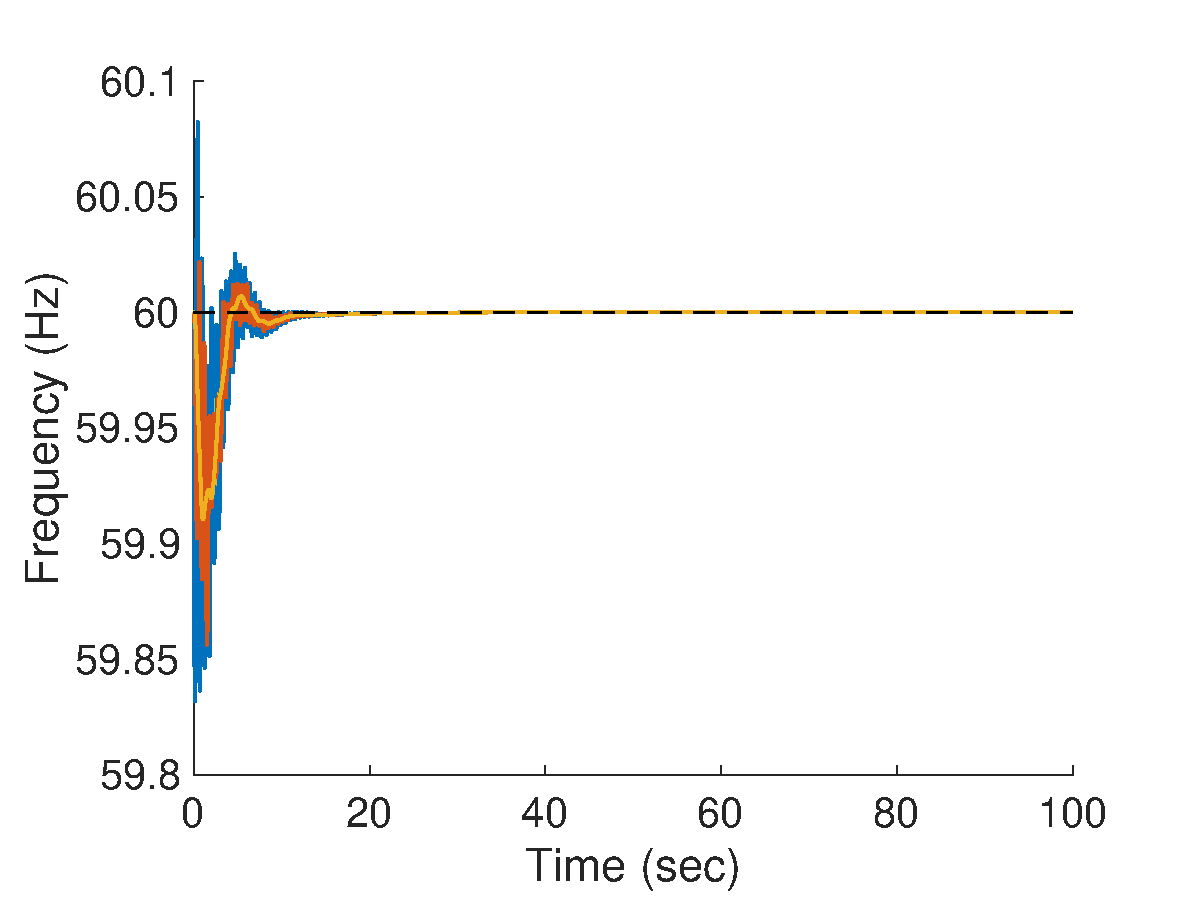
\includegraphics[width=0.3\linewidth]{figures/FrequencyWOC.eps}
		%	\caption{Frequency without congestion management}
		\label{fig:freqWOC}
}
	\subfigure[]{
		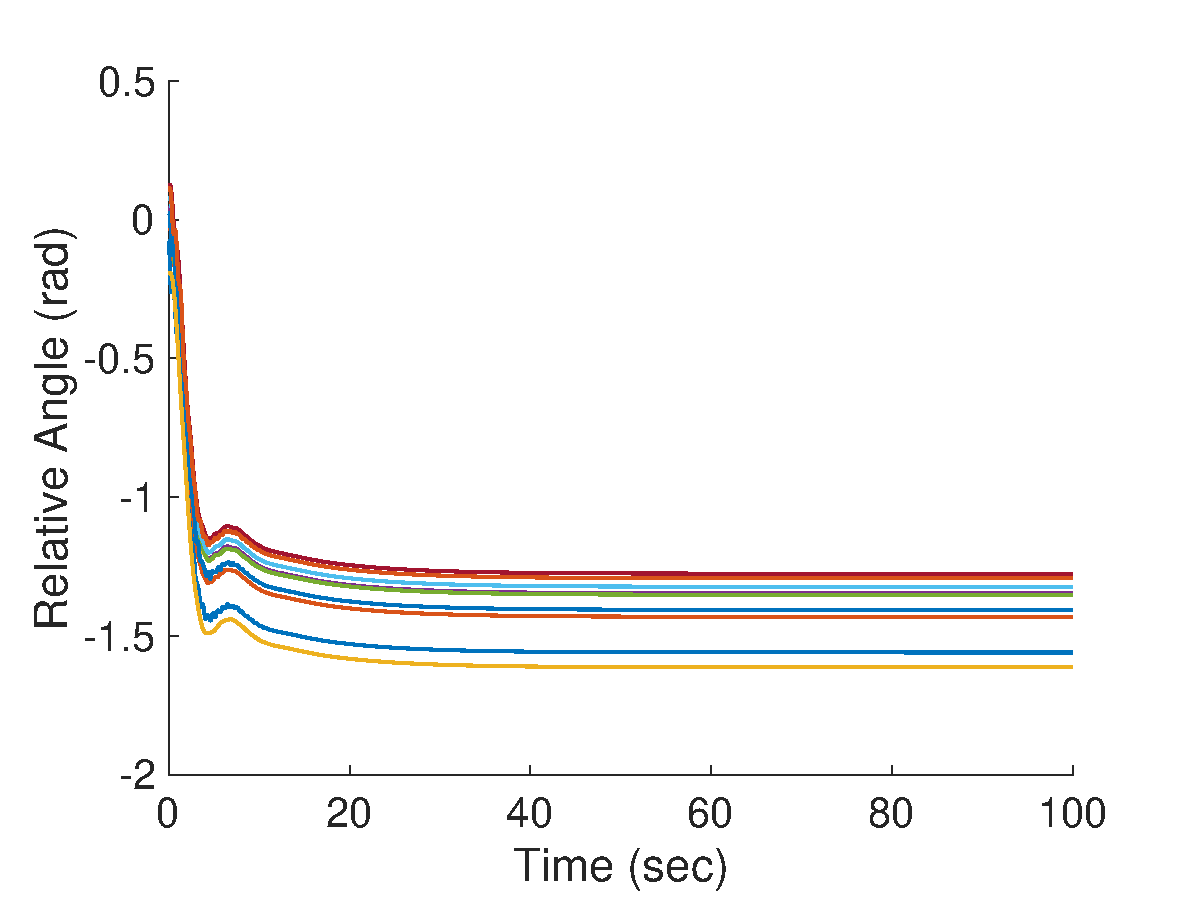
\includegraphics[width=0.3\linewidth]{figures/RelativeAngleWOC.eps}
		%	\caption{Frequency with congestion management}
		\label{fig:angleWOC}
}
	\subfigure[]{
	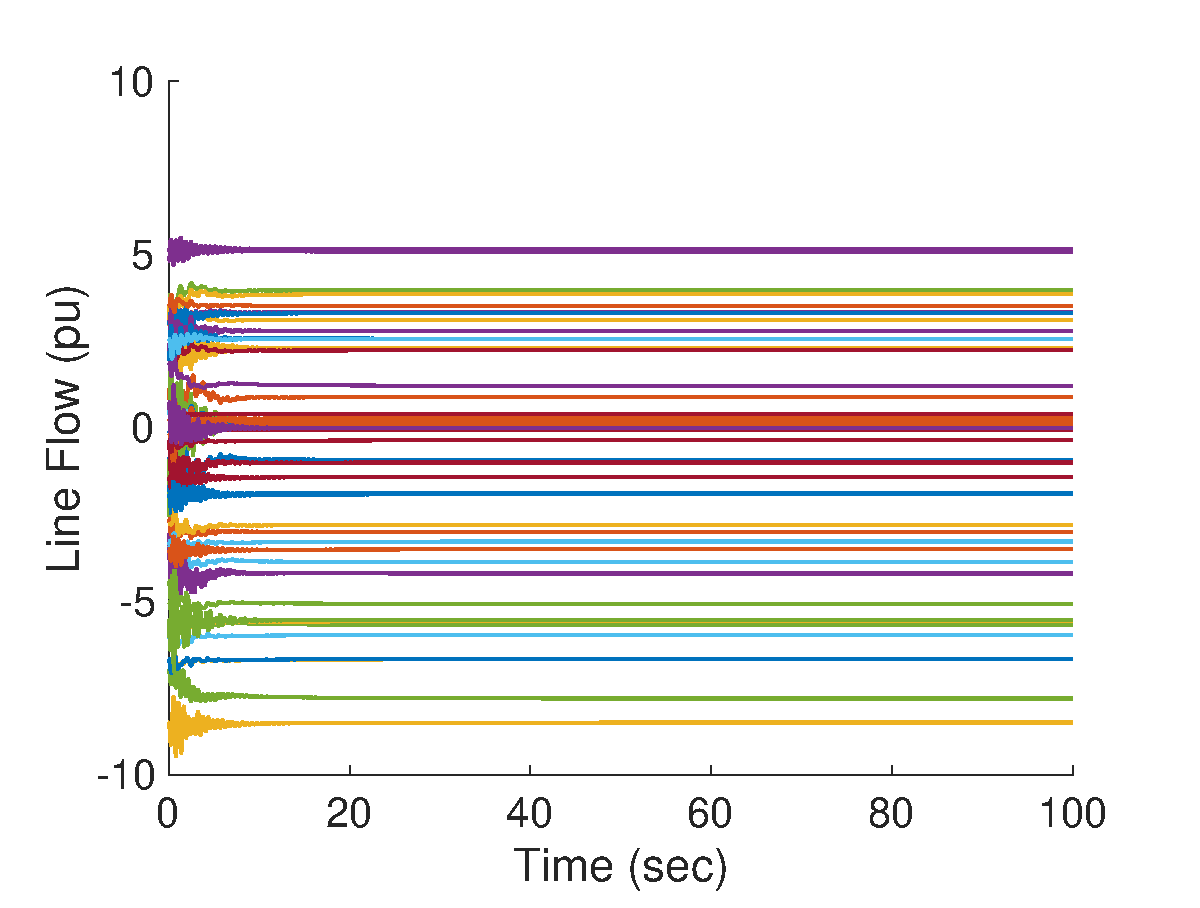
\includegraphics[width=0.3\linewidth]{figures/LineFlowWOC.eps}
	%	\caption{Frequency with congestion management}
	\label{fig:lineflowWOC}
}
	\subfigure[]{
		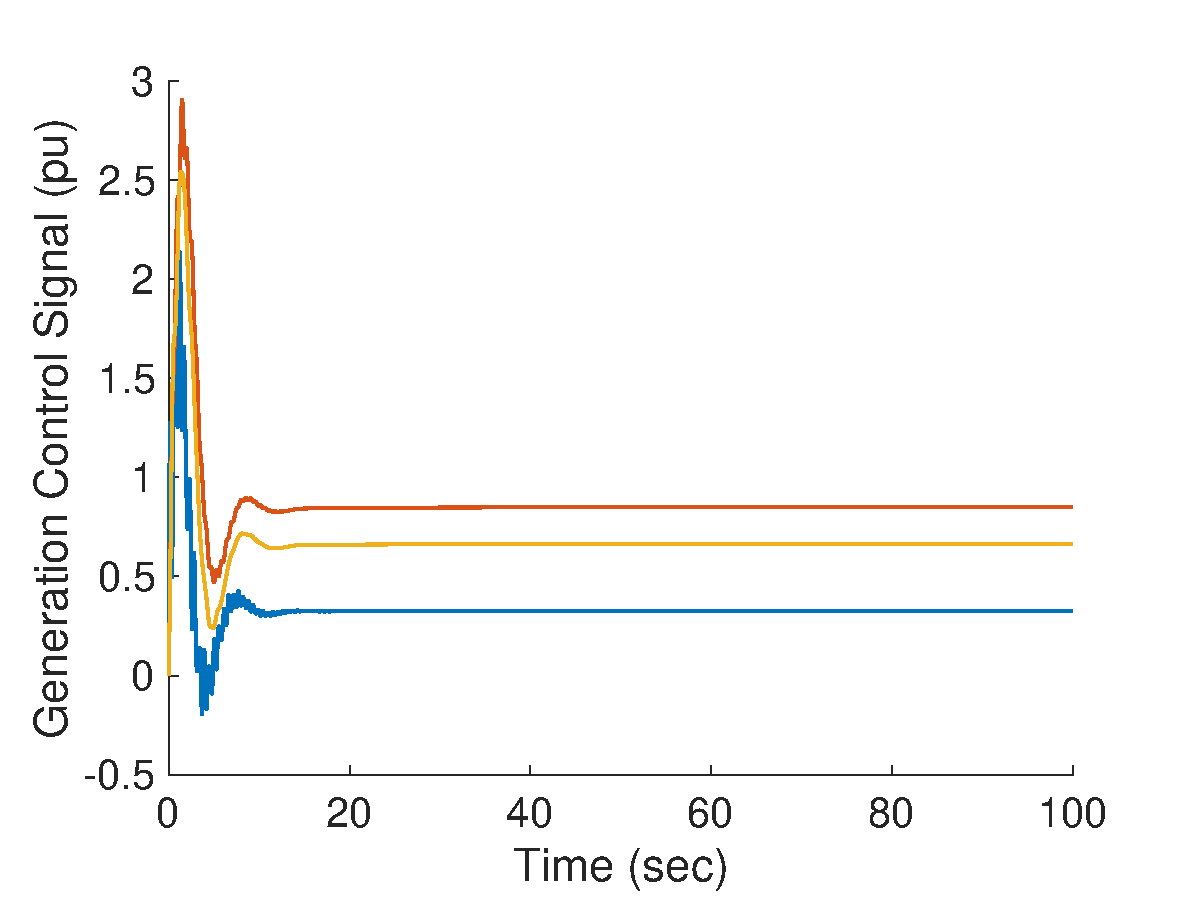
\includegraphics[width=0.3\linewidth]{figures/GenerationControlSignalWOC.eps}
		%	\caption{Frequency with congestion management}
		\label{fig:gensignalWOC}
}
	\subfigure[]{
		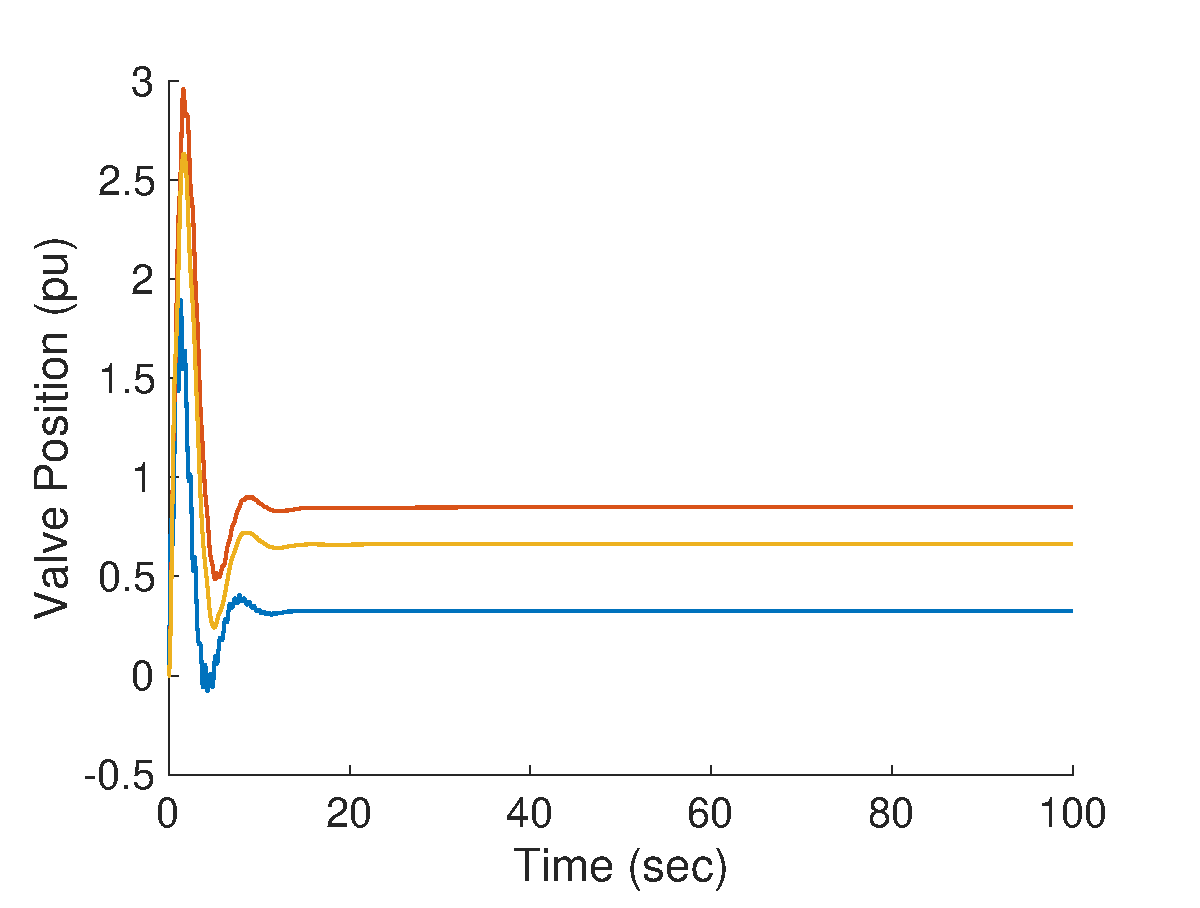
\includegraphics[width=0.3\linewidth]{figures/ValvePositionWOC.eps}
		%	\caption{Frequency with congestion management}
		\label{fig:valveWOC}
}
	\subfigure[]{
		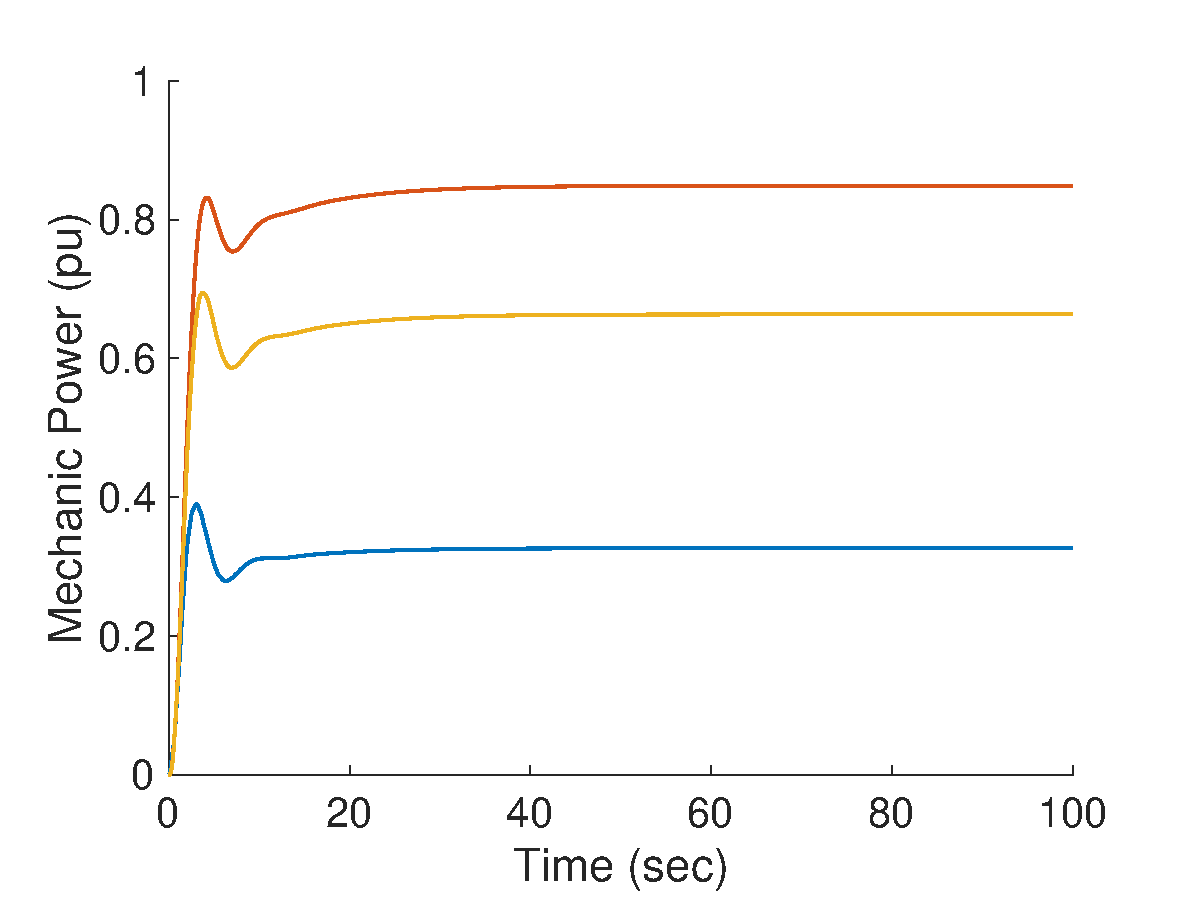
\includegraphics[width=0.3\linewidth]{figures/MechanicalPowerWOC.eps}
		%	\caption{Frequency with congestion management}
		\label{fig:genWOC}
}
	\subfigure[]{
		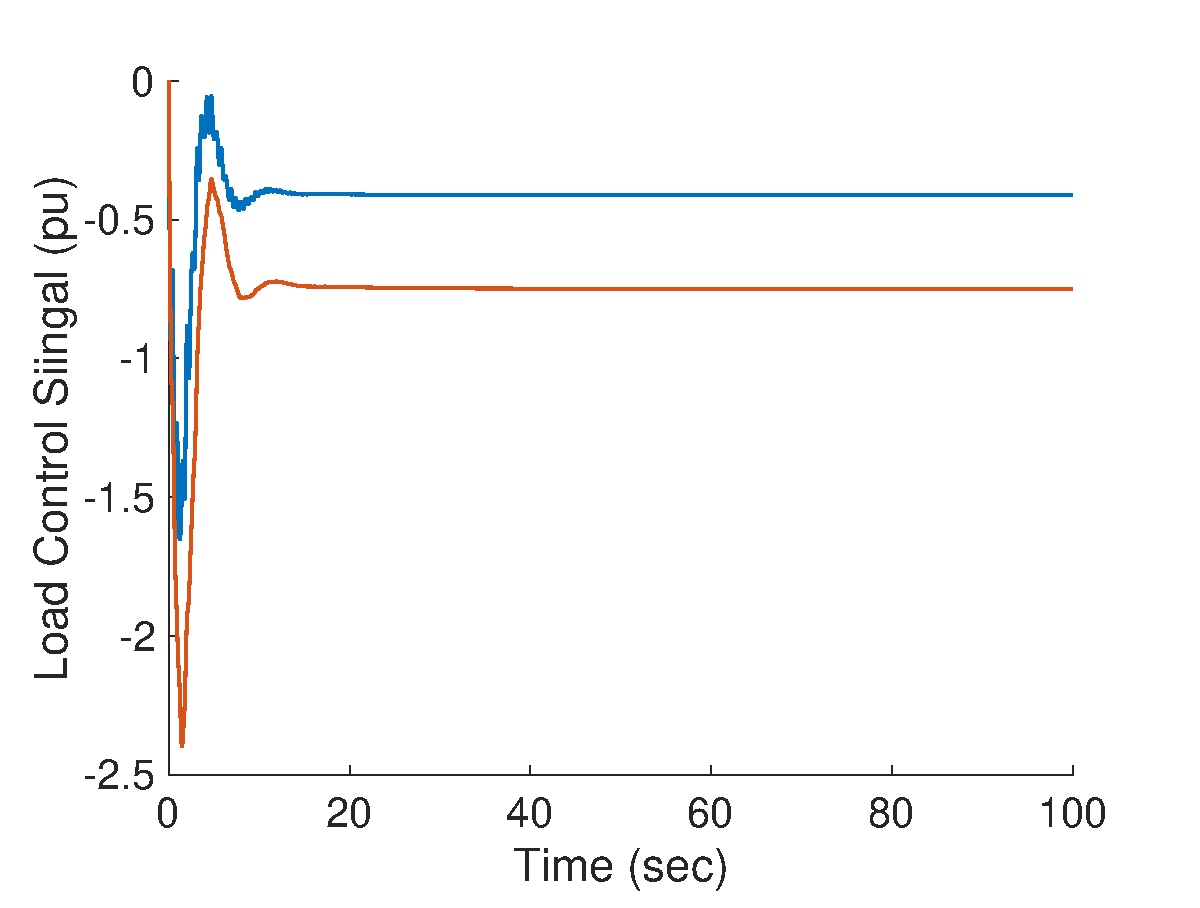
\includegraphics[width=0.3\linewidth]{figures/LoadControlSignalWOC.eps}
		%	\caption{Frequency with congestion management}
		\label{fig:loadsignalWOC}
}
	\subfigure[]{
		\includegraphics[width=0.3\linewidth]{figures/ControllableLoadWOC.eps}
		%	\caption{Frequency with congestion management}
		\label{fig:loadWOC}
}
	\caption{Dynamics without congestion management (a) Frequencies; (b) Relative phase angles; (c) Actual line flows; (d) Generation control signals; (e) Valve positions; (f) Generations; (g) Load control signals; (h) Loads.  }
	\label{fig:WOcongestion}
\end{figure}




\begin{figure}[]
	\centering
	\subfigure[]{
		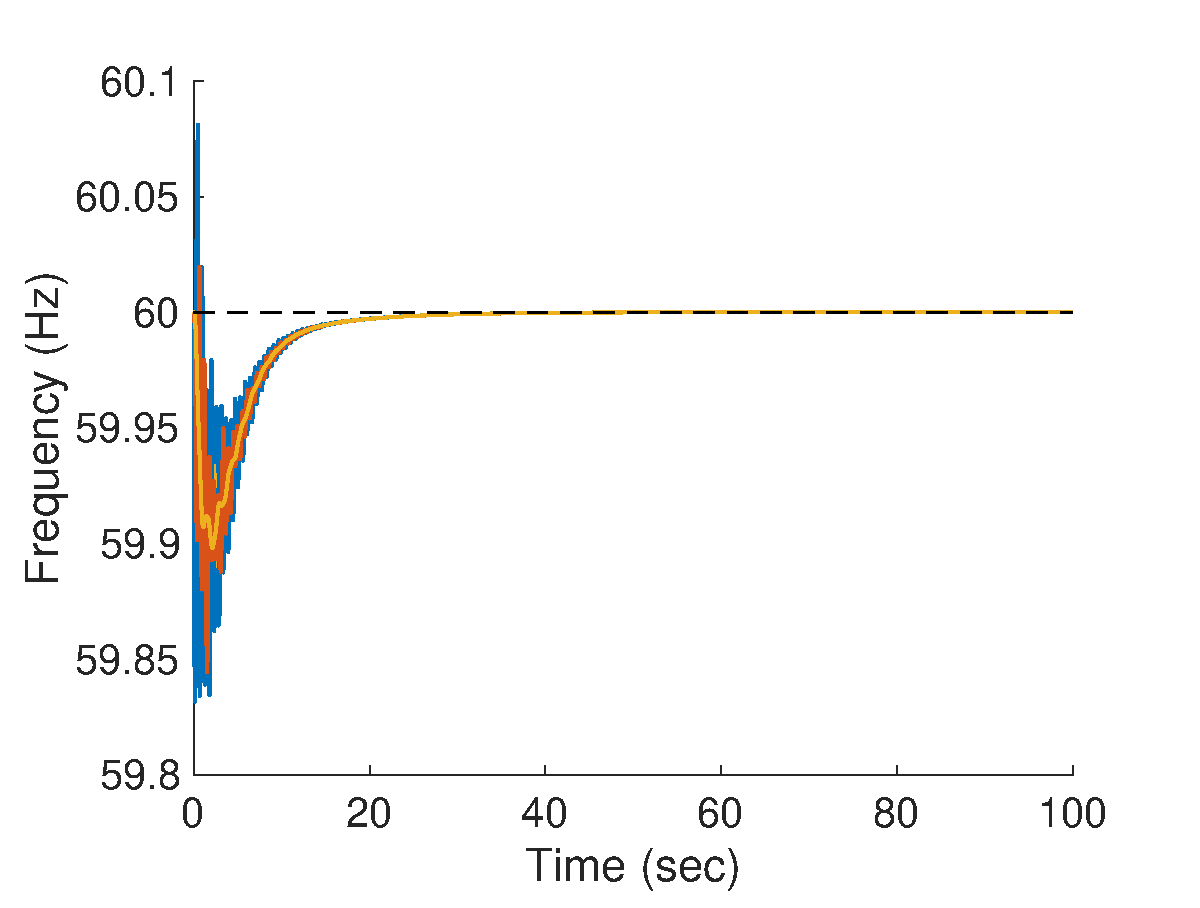
\includegraphics[width=0.3\linewidth]{figures/FrequencyWC.eps}
		%	\caption{Frequency without congestion management}
		\label{fig:freqWC}
}
	\subfigure[]{
		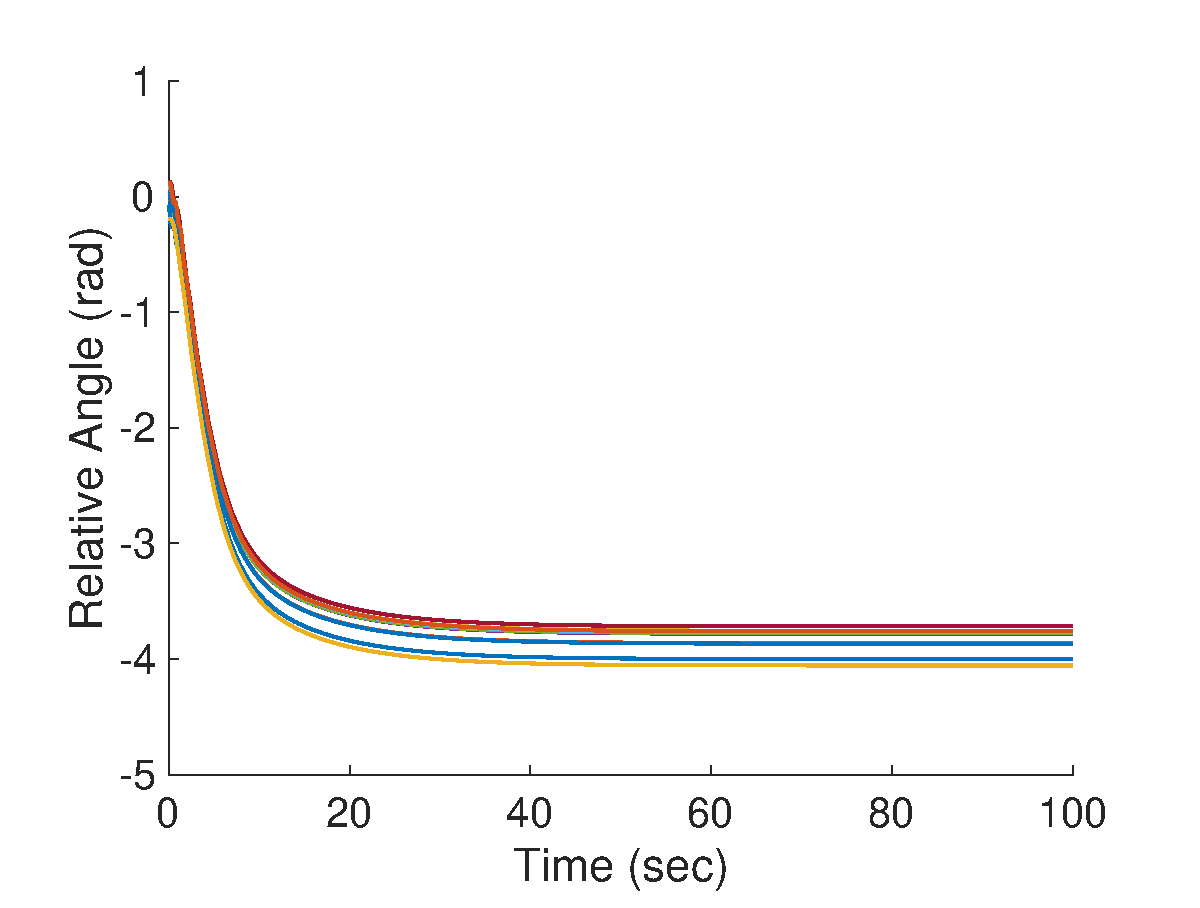
\includegraphics[width=0.3\linewidth]{figures/RelativeAngleWC.eps}
		%	\caption{Frequency with congestion management}
		\label{fig:angleWC}
}
	\subfigure[]{
		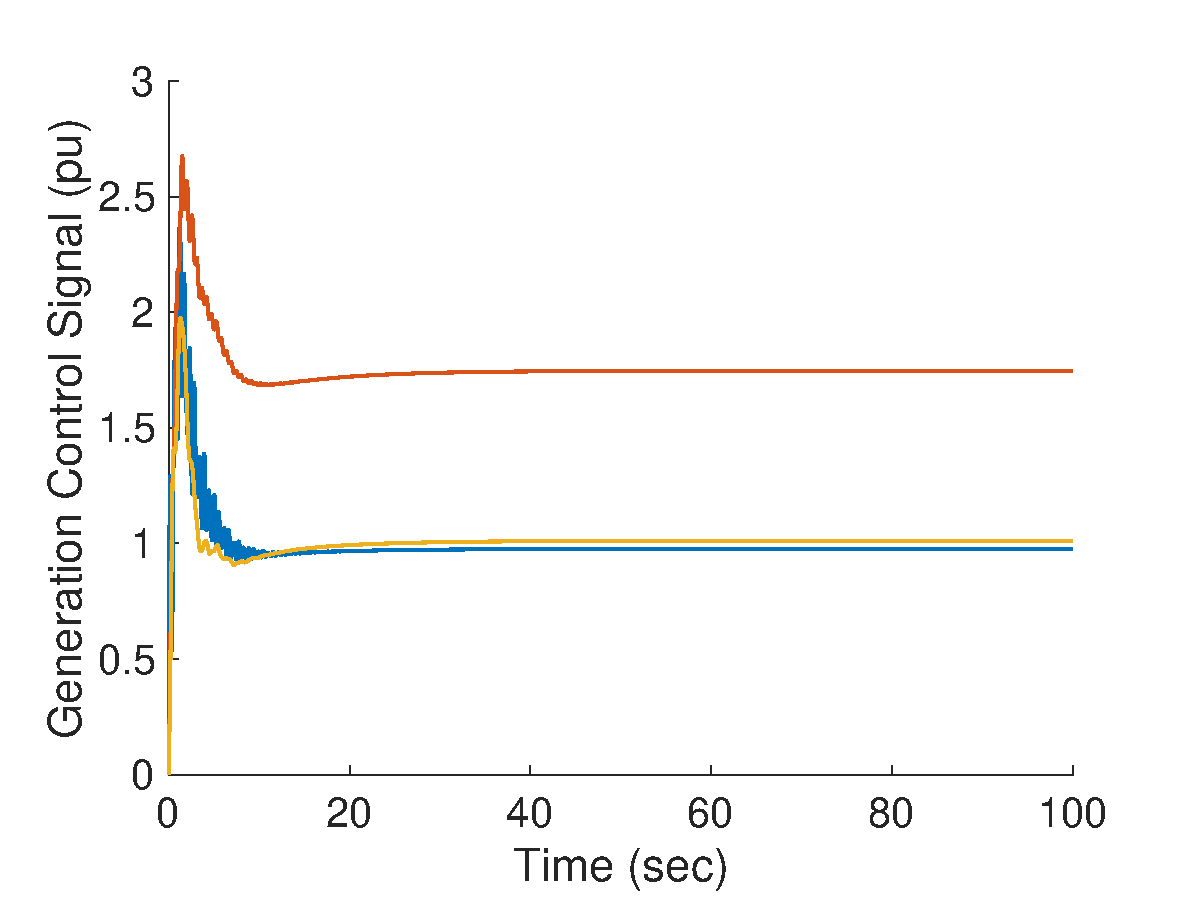
\includegraphics[width=0.3\linewidth]{figures/GenerationControlSignalWC.eps}
		%	\caption{Frequency with congestion management}
		\label{fig:gensignalWC}
}
	\subfigure[]{
		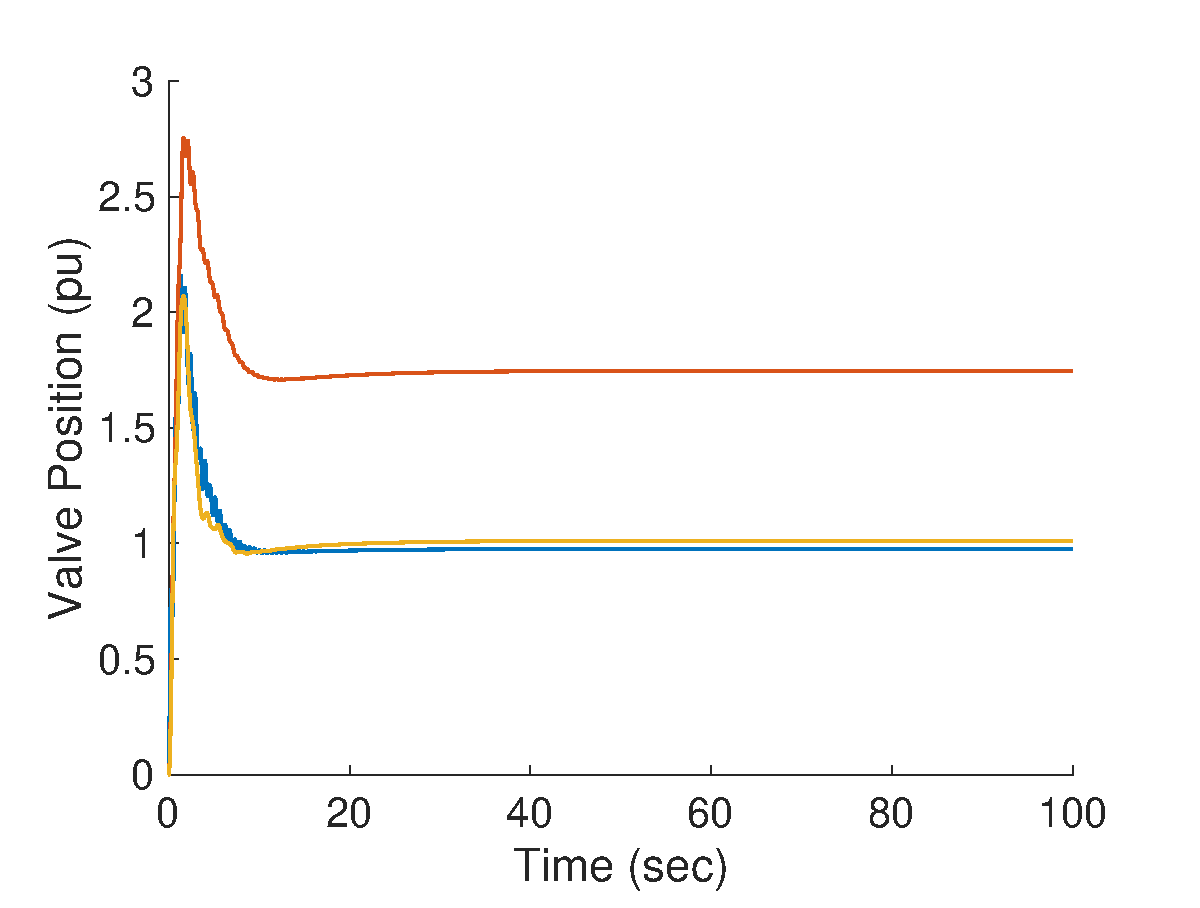
\includegraphics[width=0.3\linewidth]{figures/ValvePositionWC.eps}
		%	\caption{Frequency with congestion management}
		\label{fig:valveWC}
}
	\subfigure[]{
		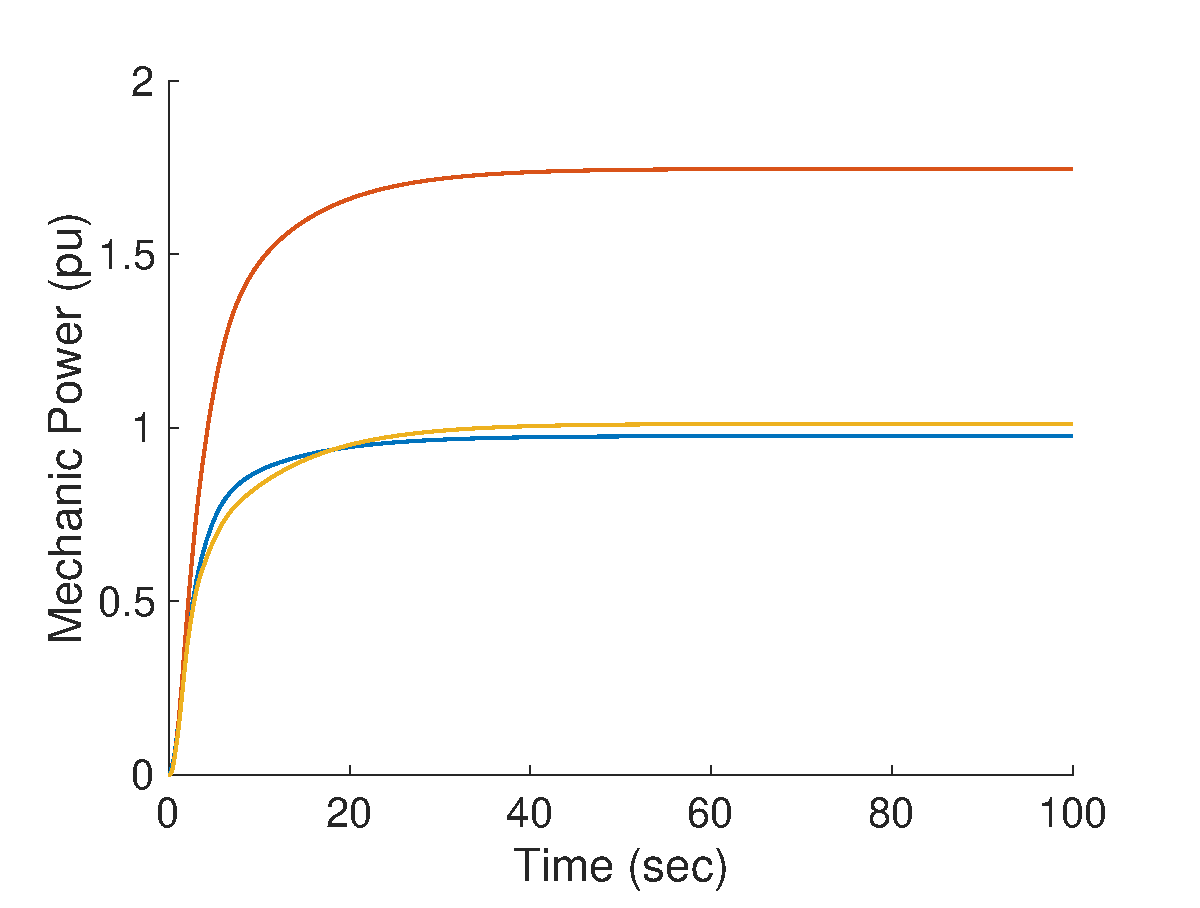
\includegraphics[width=0.3\linewidth]{figures/MechanicalPowerWC.eps}
		%	\caption{Frequency with congestion management}
		\label{fig:genWC}
}
	\subfigure[]{
		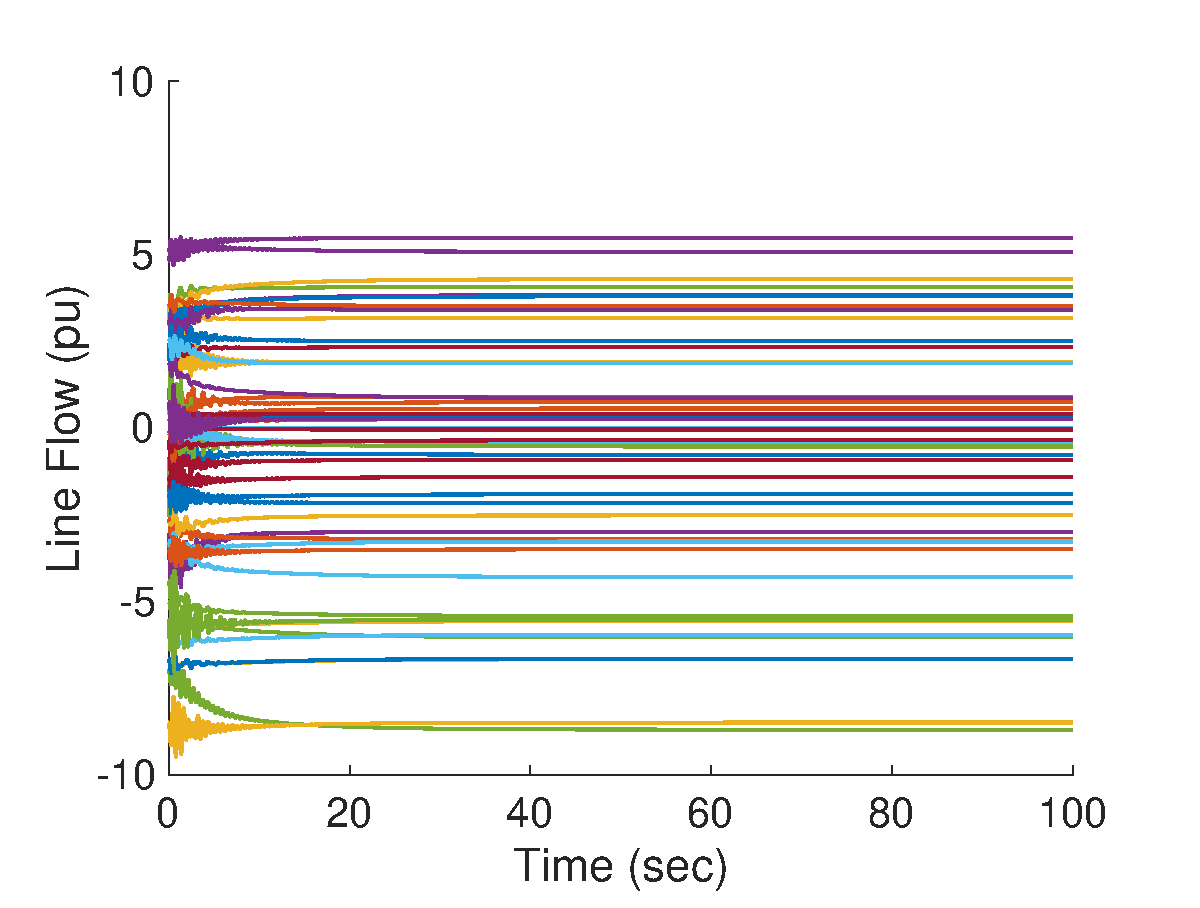
\includegraphics[width=0.3\linewidth]{figures/LineFlowWC.eps}
		%	\caption{Frequency with congestion management}
		\label{fig:lineflowWC}
}
	\subfigure[]{
		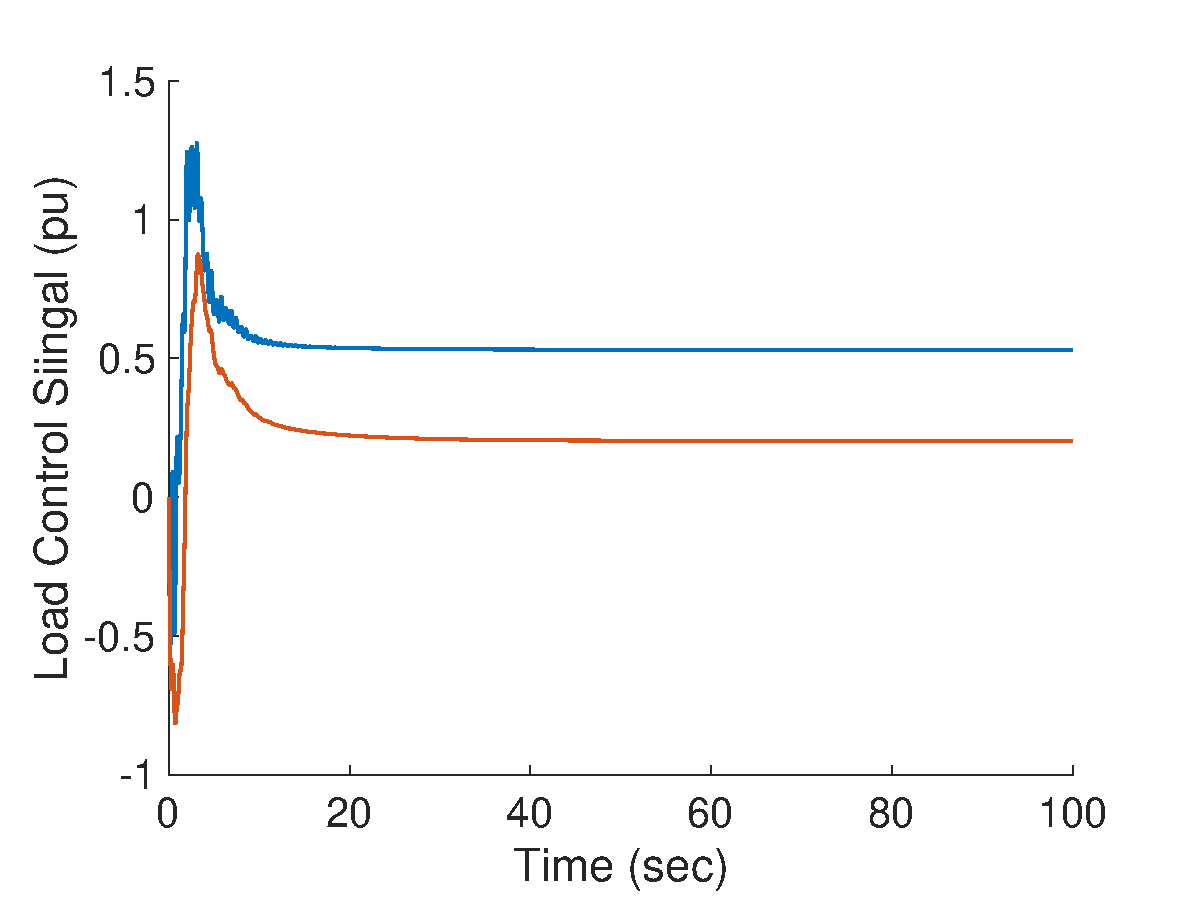
\includegraphics[width=0.3\linewidth]{figures/LoadControlSignalWC.eps}
		%	\caption{Frequency with congestion management}
		\label{fig:loadsignalWC}
}
	\subfigure[]{
		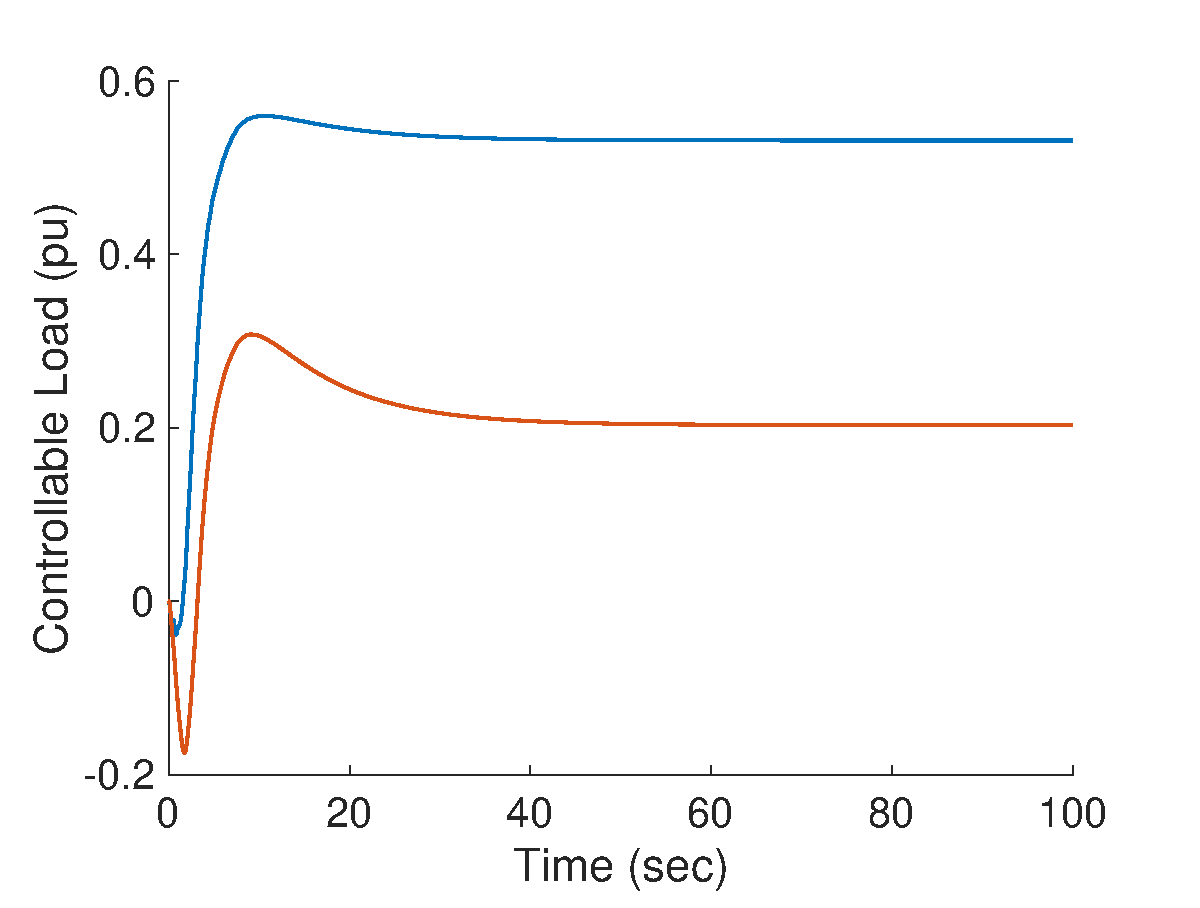
\includegraphics[width=0.3\linewidth]{figures/ControllableLoadWC.eps}
		%	\caption{Frequency with congestion management}
		\label{fig:loadWC}
}
	\caption{Dynamics with congestion management (a) Frequencies; (b) Relative phase angles; (c) Actual line flows; (d) Generation control signals; (e) Valve positions; (f) Generations; (g) Load control signals; (h) Loads.}
	\label{fig:Wcongestion}
\end{figure}








\newpage
\appendix
\section{Appendix}

\subsection{Derivation of $B$}

Here all variables are in their nominal values. Deviations will be represented by adding $\Delta$.
Consider the generic expression for a real line flow $P_{jk}$:
\begin{eqnarray}\label{eq:app:1}
     P_{jk}= |V_j||V_k|\left(-g_{jk}\cos(\theta_j-\theta_k)-b_{jk}\sin(\theta_j-\theta_k)\right)
\end{eqnarray} 
where $g_{jk}:=\frac{r_{jk}}{r_{jk}^2+x_{jk}^2}$ and $b_{jk}:=\frac{-x_{jk}}{r_{jk}^2+x_{jk}^2}$ denote the corresponding conductance and susceptance of line $(j,k)$, respectively. By the second assumption, \eqref{eq:app:1} reduces to
\begin{eqnarray}\label{eq:app:2}
P_{jk}= \frac{|V_j||V_k|}{x_{jk}}\sin(\theta_j-\theta_k)
\end{eqnarray} 
If there is a disturbance in phase angels, the line flow evolves accordingly:
\begin{eqnarray}\label{eq:app:3}
P_{jk} + \Delta P_{jk}= \frac{|V_j||V_k|}{x_{jk}}\sin((\theta_j+\Delta \theta_j)-(\theta_k+\Delta \theta_k))
\end{eqnarray} 
By applying the Taylor series to the right-hand side at the nominal phase angles and ignoring the high-order terms, we can rewrite \eqref{eq:app:3} as 
 \begin{eqnarray}\label{eq:app:4}
  P_{jk} + \Delta P_{jk}= \frac{|V_j||V_k|}{x_{jk}}\left[\sin(\theta_j-\theta_k)+\cos(\theta_j-\theta_k)(\Delta \theta_j-\Delta \theta_k)\right]
  \end{eqnarray} 
Combining \eqref{eq:app:3} and \eqref{eq:app:4} leads to the linearized line flow model in \eqref{eq:nwdym}:
 \begin{eqnarray}\label{eq:app:5}
\Delta P_{jk}= \frac{|V_j||V_k|}{x_{jk}}\cos(\theta_j-\theta_k)(\Delta \theta_j-\Delta \theta_k)
\end{eqnarray} 
where $B_{jk}:=\frac{|V_j||V_k|}{x_{jk}}\cos(\theta_j-\theta_k)$.
\qed



\subsection{Proof of Theorem \ref{teo:opm}}

With Assumption \ref{asp:feasiblity2}, there exists an finite solution to EDP-3. Since all its constraints are affine, Slater's condition is satisfied and strong duality holds. The KKT conditions are then both sufficient and necessary to characterize the primal-dual optimal solutions to EDP-3. Therefore, $x^*,\nu^*,\eta^*$ is primal dual optimal if and only if
\begin{itemize}
\item \emph{Primal feasibility}: \eqref{eq:ed3:2}-\eqref{eq:ed3:7}.
\item \emph{Dual feasibility}: $\eta^{-*},\eta^{+*}\ge 0$.
\item \emph{Stationarity}: 
\begin{displaymath}
\nabla_p L(x^*,\nu^*,\eta^*)=0,~\nabla_d L(x^*,\nu^*,\eta^*)=0,~\nabla_{\tilde{\theta}} L(x^*,\nu^*,\eta^*)=0,~\nabla_\omega L(x^*,\nu^*,\eta^*)=0.
\end{displaymath}
\item \emph{Complementary slackness}: \eqref{eq:opm:4}, \eqref{eq:opm:5}.
\end{itemize}  

The first two stationarity conditions give \eqref{eq:opm:2}, \eqref{eq:opm:3}. The third stationarity condition requires
\begin{equation}
    \frac{\partial L}{\partial \tilde \theta_{jk} }(x^*,\nu^*,\eta^*) = B_{jk} (\mu_j^*-\mu_k^*)= 0,\quad (j,k)\in\mathcal{E}
\end{equation}
%Note that if $j=0$ or $k=0$, then $\mu_j^*=0$ or $\mu_k^*=0$ as it is not defined\footnote{Actually here we can already obtain $\mu^*=\mathbf{0}$ ($\omega^*_{\mathcal{N}^+}=\mathbf{0}$) thanks to our assumption that $\theta_0=0$ at bus 0. However, we would like to show this property always holds even without the assumption.}.
Considering $B_{jk} >0$, $\mu^*_j=\mu^*_k$, $(j,k)\in\mathcal{E}$. Since the graph $(\mathcal{N},\mathcal{E})$ is connected, naturally $\mu^*_j=\alpha$, $j\in\mathcal{N}$, where $\alpha$ is a constant. Meanwhile, the fourth stationarity condition implies 
\beq
\frac{\partial L}{\partial \omega_j}(x^*,\nu^*,\eta^*)= D_j\omega_j^* -D_j \mu_j^* = 0,\quad j \in\mathcal{N}
\eeq
Considering $D_j>0$, $\mu_j^*=\omega_j^*$, $j\in\mathcal{N}$. Therefore, $\omega_j=\alpha$, $j\in\mathcal{N}$, as well.

From \eqref{eq:ed3:5} and the above observation, summing up \eqref{eq:ed3:2}-\eqref{eq:ed3:4} over rows leads to $\sum_{j\in\mathcal{N}} D_j\omega_j = \alpha \sum_{j\in\mathcal{N}} D_j=0$, which implies $\alpha = 0$, i.e., $\mu^*=\omega^*={0}$ as \eqref{eq:opm:1} suggests. Therefore, the KKT conditions are fully captured in Theorem \ref{teo:opm}.     
\qed  


\subsection{Proof of Theorem \ref{teo:equiv}}

\noindent
\textbf{EDP-1 $\rightarrow$ EDP-2}:

Given an optimal solution $(p^*,d^*,\theta^*_{\mathcal{N}^+})$ to EDP-1, assume $(p^*,d^*)$ is not an optimal solution to EDP-2. Then there exists $(\hat{p},\hat{d})$ that satisfies \eqref{eq:ed2:2}-\eqref{eq:ed2:4} and has a strict smaller objective function $\sum_{j\in\mathcal{G}}J_j(\hat p_j)-\sum_{j\in\mathcal{N}^+}U_j(\hat d_j) < \sum_{j\in\mathcal{G}}J_j( p^*_j)-\sum_{j\in\mathcal{N}^+}U_j( d^*_j) $. Let $\hat \theta_{\mathcal{N}^+} := (\bar{C}B\bar{C}^T)^{-1}\hat \pi_{\mathcal{N}^+}$ with $\hat \pi_{\mathcal{G}} =r_\mathcal{G}+\hat{p}-\hat d_\mathcal{G}$ and $\hat \pi_{\mathcal{L}}=r_\mathcal{L}-\hat d_\mathcal{L}$. It is trivial to verify that $(\hat{p},\hat{d},\hat \theta_{\mathcal{N}^+})$ satisfies \eqref{eq:ed:2}-\eqref{eq:ed:5} and is thus feasible for EDP-1 with a strict smaller objective function than $(p^*,d^*,\theta^*_{\mathcal{N}^+})$. However, this contradicts with the fact that $(p^*,d^*,\theta^*_{\mathcal{N}^+})$ is optimal with respect to EDP-1. Therefore, $(p^*,d^*)$ is an optimal solution to EDP-2. 

\noindent
\textbf{EDP-2 $\rightarrow$ EDP-3}:

Given an optimal solution $(p^*,d^*)$ to EDP-2, assume $(p^*,d^*, \tilde \theta^*=\bar{C}^T(\bar{C}B\bar{C}^T)^{-1}\pi_{\mathcal{N}^+}^*,\omega^*=0)$ is not an optimal solution to EDP-3. Then there exists $(\hat p,\hat d, \hat{\tilde \theta}=\bar{C}^T(\bar{C}B\bar{C}^T)^{-1}\hat \pi_{\mathcal{N}^+},\hat \omega=0)$ that satisfies \eqref{eq:ed3:2}-\eqref{eq:ed3:7} and has a strict smaller objective function $\sum_{j\in\mathcal{G}}J_j(\hat p_j)-\sum_{j\in\mathcal{N}^+}U_j(\hat d_j) < \sum_{j\in\mathcal{G}}J_j( p^*_j)-\sum_{j\in\mathcal{N}^+}U_j( d^*_j) $. Note that ${\tilde{\theta}}$ is a function of $p$ and $d$, thus $\hat{\tilde \theta}$ may still equal $\tilde\theta^*$ despite $(\hat{p},\hat{d}) \neq (p^*,d^*)$. Apparently $(\hat{p},\hat{d})$ satisfies \eqref{eq:ed2:2}-\eqref{eq:ed2:4} (the same as \eqref{eq:ed3:5}-\eqref{eq:ed3:7}) and is thus feasible for EDP-2 with a strict smaller objective function than $(p^*,d^*)$. However, this contradicts with the fact that $(p^*,d^*)$ is optimal with respect to EDP-2. Therefore, $(p^*,d^*, \tilde \theta^*=\bar{C}^T(\bar{C}B\bar{C}^T)^{-1}\pi_{\mathcal{N}^+}^*,\omega^*=0)$ is an optimal solution EDP-3.

\noindent\textbf{EDP-3 $\rightarrow$ EDP-1}:

Given an optimal solution $(p^*,d^*, \tilde \theta^*,\omega^*=0)$ to EDP-3, assume $(p^*,d^*,\theta_{\mathcal{N}^+}^*)$ is not an optimal solution to EDP-1 for arbitrary $\theta_{\mathcal{N}^+}^*$ that satisfies $\tilde\theta^*=\bar{C}^T \theta_{\mathcal{N}^+}^*$. Then there exists $(\hat{p},\hat{d},\hat \theta_{\mathcal{N}^+})$ that satisfies \eqref{eq:ed:2}-\eqref{eq:ed:5} and has a strict smaller objective function $\sum_{j\in\mathcal{G}}J_j(\hat p_j)-\sum_{j\in\mathcal{N}^+}U_j(\hat d_j) < \sum_{j\in\mathcal{G}}J_j( p^*_j)-\sum_{j\in\mathcal{N}^+}U_j( d^*_j)$. Note that $\hat{\tilde{\theta}}:=\bar{C}^T \hat \theta_{\mathcal{N}^+}$ may still equal $\tilde \theta^*$ despite $(\hat{p},\hat{d}) \neq (p^*,d^*)$. It follows from \eqref{eq:ed:2}-\eqref{eq:ed:4} that $(\hat{p},\hat{d},\hat{\tilde{\theta}},\hat \omega=0)$ satisfies \eqref{eq:ed3:2}-\eqref{eq:ed3:4} and naturally \eqref{eq:ed3:5} by summing \eqref{eq:ed3:2}-\eqref{eq:ed3:4} up. Write $\hat\theta_{\mathcal{N}^+}$ in terms of $\hat{p}$ and $\hat{d}$ as $\hat\theta_{\mathcal{N}^+}=(\bar{C}B\bar{C}^T)^{-1}\hat \pi_{\mathcal{N}^+}$, where $\hat \pi_{\mathcal{G}} =r_\mathcal{G}+\hat{p}-\hat d_\mathcal{G}$ and $\hat \pi_{\mathcal{L}}=r_\mathcal{L}-\hat d_\mathcal{L}$, then it follows from \eqref{eq:ed:5} that $(\hat{p},\hat{d},\hat{\tilde{\theta}},\hat \omega=0)$ also satisfies \eqref{eq:ed3:6}, \eqref{eq:ed3:7}. Therefore, $(\hat{p},\hat{d},\hat{\tilde{\theta}},\hat \omega=0)$ is feasible for EDP-3 with a strict smaller objective function than $(p^*,d^*, \tilde \theta^*,\omega^*=0)$, which however is already optimal with respect to EDP-3. The contradiction indicates that $(p^*,d^*,\theta_{\mathcal{N}^+}^*)$ is an optimal solution to EDP-1 for arbitrary $\theta_{\mathcal{N}^+}^*$ that satisfies $\tilde\theta^*=\bar{C}^T \theta_{\mathcal{N}^+}^*$.  



\qed

\subsection{Proof of Theorem \ref{teo:eqlb}}

\noindent
\textbf{Necessary condition}:

Given an equilibrium point $(p^*,d^*,\theta^*,\omega^*,\lambda^*,\eta^{-*},\eta^{+*})$,
$\{\dot{\theta}=0, \dot{\omega}=0\} \leftrightarrow \eqref{eq:opm:1}$, 
$\dot{p}=0 \leftrightarrow \eqref{eq:opm:2}$ and $\dot{d}=0 \leftrightarrow \eqref{eq:opm:3}$. Therefore, the stationarity conditions are satisfied.

With $\omega^*=\mu^*=0$ and $\dot{\omega}=\dot{\mu}=0$, \eqref{eq:nwdymvec:2}-\eqref{eq:nwdymvec:4} imply \eqref{eq:ed3:2}-\eqref{eq:ed3:4}, respectively, if we set $\tilde{\theta}^*=C^T \theta^*$. In addition, $\dot \lambda =0 \leftrightarrow \eqref{eq:ed3:5}$. By the definition of $[\cdot]^+_\eta$, $\dot \eta^- =0$ and $\dot \eta^+=0$ imply \eqref{eq:ed3:6} and \eqref{eq:ed3:7}, respectively. Therefore, the equilibrium point is primal feasible.

Note that the trajectory starts from an initial point in $\mathbb{I}$, then the definition of $[\cdot]^+_\eta$ enforces $\eta^-(t),\eta^+(t)\ge 0$ for all $t\ge 0$. On this basis, dual feasibility is guaranteed.

Finally, we have \eqref{eq:ed3:6} with primal feasibility. If the equality sign holds, \eqref{eq:opm:4} is satisfied. If the strict less-than sign holds, $\eta^-$ will be driven to $0$, thus satisfying \eqref{eq:opm:4} as well. A similar argument applies to \eqref{eq:opm:5}. Therefore, the complementary slackness conditions are also met. 

From above, $(p^*,d^*,\tilde{\theta}^*,\omega^*,\mu^*,\lambda^*,\eta^{-*},\eta^{+*})$ is a primal-dual optimal solution to EDP-3.   


 
\noindent
\textbf{Sufficient condition}:
 
Given a primal-dual optimal solution $(p^*,d^*,\tilde{\theta}^*,\omega^*,\mu^*,\lambda^*,\eta^{-*},\eta^{+*})$ to EDP-3, as we have shown above, the stationarity conditions \eqref{eq:opm:1}-\eqref{eq:opm:3} imply $\dot{\theta}=0$, $\dot \omega =0$, $\dot p =0$ and $\dot d=0$. Then the primal feasibility condition \eqref{eq:ed3:5} implies $\dot \lambda = 0$. Finally, we have \eqref{eq:ed3:6} with primal feasibility. If the equality sign holds, $\dot \eta^- =0$. If the less-than sign holds, $\eta^{-*}=0$ according to the complementary slackness condition \eqref{eq:opm:4}. Still we have $\dot \eta^- =0$. A similar argument applies to $\dot \eta^+ =0$.

From above, $(p^*,d^*,\theta^*,\omega^*,\lambda^*,\eta^{-*},\eta^{+*})$ is an equilibrium point.  

\qed


\subsection{Proof of Theorem \ref{teo:stability}}
	
	Consider the following Lyapunov function 
	\beq
	V(\tilde x, \tilde \nu, \eta) = \frac{1}{2} (\tilde{x}-\tilde x^* )^T {\Gamma^{\tilde{x}}}^{-1} (\tilde{x}-\tilde x^* ) + \frac{1}{2} (\tilde{\nu}-\tilde \nu^* )^T {\Gamma^{\tilde{\nu}}}^{-1} (\tilde{\nu}-\tilde \nu^* ) +  \frac{1}{2} (\eta-\eta^* )^T {\Gamma^{\eta}}^{-1}(\eta-\eta^* )
	\eeq
	where $\Gamma^{\tilde{x}}:=\diag(\gamma^p_{\mathcal{G}}, \gamma^d_{\mathcal{N}^+},\gamma^{\tilde\theta}_{\mathcal{E}})$, $\Gamma^{\tilde{\nu}}:=\diag( \gamma^\mu_\mathcal{G},\gamma^\lambda)$ and $\Gamma^\eta:=\diag(\gamma^{\eta^-}_\mathcal{E},\gamma^{\eta^+}_\mathcal{E})$. Its derivative with respect to time is 
	\beq
	\begin{split}
		\dot V(\tilde x, \tilde \nu,\eta) = & -\nabla_{\tilde x}{ L} (\tilde x, \tilde \nu,\eta)^T(\tilde{x}-\tilde x^* ) + \nabla_{ \tilde \nu} L (\tilde x, \tilde \nu,\eta)^T(\tilde{\nu}-\tilde \nu^* )+  {\left[\nabla_{\eta} L(\tilde x, \tilde \nu,\eta)\right ]^+_{\eta}}^T (\eta- \eta^*) \\
		\le & -\nabla_{\tilde x}{ L} (\tilde x, \tilde \nu,\eta)^T(\tilde{x}-\tilde x^* ) + \nabla_{ \tilde \nu} L (\tilde x, \tilde \nu,\eta)^T(\tilde{\nu}-\tilde \nu^* )+  {\nabla_{\eta} L(\tilde x, \tilde \nu,\eta)}^T (\eta- \eta^*)  \\
		\le &   L(\tilde{x}^*, \tilde \nu, \eta) - L(\tilde{x},\tilde{\nu},\eta) +  L(\tilde{x},\tilde{\nu},\eta) - L(\tilde x,\tilde{\nu}^*,\eta^*) \\
		= &   L(\tilde{x}^*, \tilde \nu, \eta) - L(\tilde{x}^*,\tilde{\nu}^*,\eta^*) +  L(\tilde{x}^*,\tilde{\nu}^*,\eta^*) - L(\tilde x,\tilde{\nu}^*,\eta^*) \\
		\le & 0
	\end{split}
	\eeq
	The first equality applies \eqref{eq:pdalg}. The second inequality holds due to the fact that ${[y]_u^+}^T (u-u^*)\le y^T(u-u^*)$ for arbitrary vectors $y$, $u$ and $u^*\ge 0$. The third inequality arises from the convexity of $L(\tilde{x},\tilde{\nu},\eta)$ with respect to $\tilde{x}$ and its concavity with respect to $(\tilde{\nu},\eta)$. The last inequality holds since the equilibrium point $(\tilde{x}^*,\tilde{\nu}^*,\eta^*)$ is also a saddle point of $L(\tilde{x},\tilde{\nu},\eta)$.
	
	Define the largest invariant set between the on-off switches of the projection $[\cdot]_\eta^+$ by 
	\beq
	\mathbb{S}:=\left\{  (\tilde x, \tilde \nu, \eta) \ | \ \dot{V}(\tilde x(t), \tilde \nu(t), \eta(t)) = 0 ,\   t\ge \max\{ t^-_{jk},t^+_{jk}, (j,k)\in\mathcal{E}\} \right\}
	\eeq
	where $t_{jk}^-$ and $t_{jk}^+$ are the time epochs when the projections corresponding to $\eta_{jk}^-$ and $\eta_{jk}^+$ switch between on and off, respectively. Since the Lyapunov function is radially unbounded, the trajectories will remain bounded. Moreover, as per the invariance principle for Caratheodory systems \cite{bacciotti2006nonpathological}, $(\tilde x(t), \tilde \nu(t), \eta(t))$ converges to $\mathbb{S}$ as $t\rightarrow \infty$.
	
	For any trajectory $(\tilde x(t), \tilde \nu(t), \eta(t))\in\mathbb{S}$, $\dot V {(\tilde x(t), \tilde \nu(t), \eta(t))} = 0$ enforces
	\beq\label{eq:prf1}
	L(\tilde x(t),\tilde{\nu}^*,\eta^*)  = L(\tilde{x}^*,\tilde{\nu}^*,\eta^*) = L(\tilde{x}^*, \tilde \nu(t), \eta(t))
	\eeq
	Differentiating the first equality of \eqref{eq:prf1} with respect to time leads to
	\beq
	\dot L(\tilde x(t),\tilde{\nu}^*,\eta^*)=\nabla_{\tilde{x}} L(\tilde x(t),\tilde{\nu}^*,\eta^*)^T \dot{\tilde{x}}=- \nabla_{\tilde{x}} L(\tilde x(t),\tilde{\nu}^*,\eta^*)^T   \Gamma^{\tilde{x}}  \nabla_{\tilde{x}} L(\tilde x(t),\tilde{\nu}^*,\eta^*) =0
	\eeq
	Since $\Gamma^{\tilde{x}}$ is positive definite, $ \nabla_{\tilde{x}} L(\tilde x(t),\tilde{\nu}^*,\eta^*) =0$. Therein
	\beq
	\nabla_{\tilde{\theta}} L(\tilde x(t),\tilde{\nu}^*,\eta^*) = B(C_\mathcal{G}^T \mu_\mathcal{G}^* +  C_\mathcal{L}^T \mu_\mathcal{L}^*(\tilde x(t),\tilde{\nu}^*,\eta^*) +C_0^T \mu_0^* (\tilde x(t),\tilde{\nu}^*,\eta^*) ) = 0 
	\eeq
	and note that $\mu^*_{\mathcal{G}}=0$ as well as $[C_\mathcal{L}^T,C_0^T]$ is full column rank, we obtain $ \mu_\mathcal{L}^*(\tilde x(t),\tilde{\nu}^*,\eta^*) =0$ and $\mu_0^* (\tilde x(t),\tilde{\nu}^*,\eta^*) =0$. In addition, from \eqref{eq:Lagrangian2} $\mu_\mathcal{L}^*(\tilde x(t),\tilde{\nu}(t),\eta(t)) $ and $\mu_0^*(\tilde x(t),\tilde{\nu}(t),\eta(t))$ actually depend only on $\tilde{x}(t)$, i.e., $\nabla_{\tilde{\nu}}\mu_{\mathcal{G}}^*(\tilde x(t),\tilde{\nu}(t),\eta(t))=0$, $\nabla_{\eta}\mu_{\mathcal{G}}^*(\tilde x(t),\tilde{\nu}(t),\eta(t))=0$, $\nabla_{\tilde{\nu}}\mu_{0}^*(\tilde x(t),\tilde{\nu}(t),\eta(t))=0$ and $\nabla_{\eta}\mu_0^*(\tilde x(t),\tilde{\nu}(t),\eta(t))=0$, which implies $\mu_\mathcal{L}^*(\tilde x(t),\tilde{\nu}(t),\eta(t)) \equiv 0 =\mu_\mathcal{L}^* $ and $\mu_0^*(\tilde x(t),\tilde{\nu}(t),\eta(t)) \equiv 0 =\mu_0^*$.
	
	From above, $\nabla_{p} L(\tilde x(t),\tilde{\nu}^*,\eta^*)=0$ and $\nabla_{d} L(\tilde x(t),\tilde{\nu}^*,\eta^*)=0$ directly indicate
	\beq
	\begin{split}
		p_j(t) \equiv J_j'^{-1}(\lambda^*-\mu^*_j+H_j\eta^{-*}-H_j\eta^{+*}) =    p^*_j     ,\quad j\in\mathcal{G}     \\
		d_j(t) \equiv U_j'^{-1}(\lambda^*-\mu^*_j+H_j\eta^{-*}-H_j\eta^{+*})    =d^*_j      ,\quad j\in\mathcal{N}^+ 
	\end{split}
	\eeq
	
	Similarly, differentiating the second equality of \eqref{eq:prf1} with respect to time leads to 
	\beq
	\nabla_{\tilde{\nu}} L(\tilde x^*,\tilde{\nu}(t),\eta(t))^T   \Gamma^{\tilde{\nu}} \nabla_{\tilde{\nu}} L(\tilde x^*,\tilde{\nu}(t),\eta(t))  +  
	\nabla_{\eta} L(\tilde x^*,\tilde{\nu}(t),\eta(t))^T   \Gamma^{\eta} \left[\nabla_{\eta} L(\tilde x^*,\tilde{\nu}(t),\eta(t)) \right] ^+_\eta =0
	\eeq
	Since both $ \Gamma^{\tilde{\nu}} $ and $ \Gamma^{\eta}$ are positive definite and the second term on the left-hand side is nonnegative, we obtain $\nabla_{\tilde{\nu}} L(\tilde x^*,\tilde{\nu}(t),\eta(t)) =0$. Therein
	\beq\label{eq:prf2}
	\begin{split}
		\nabla_{\lambda} L(\tilde x^*,\tilde{\nu}(t),\eta(t)) =& \ - \mathbf 1^T_\mathcal{G} (r_\mathcal{G}+p^*-d^*_\mathcal{G})  - \mathbf 1^T_\mathcal{L} (r_\mathcal{L}-d^*_\mathcal{L}) -r_0 \\
		= & \ - \mathbf 1^T_\mathcal{G} (r_\mathcal{G}+p(t)-d_\mathcal{G}(t))  - \mathbf 1^T_\mathcal{L} (r_\mathcal{L}-d_\mathcal{L}(t)) -r_0 \\
		= &\ \frac{\dot \lambda}{\gamma^\lambda} \\
		=& \ 0
	\end{split}
	\eeq
	As a consequence, $\dot \lambda = 0 $ and $\lambda(t) \equiv \hat{\lambda}$ for some constant $\hat{\lambda}$. Moreover, $\nabla_{\mu_\mathcal{G}} L(\tilde x^*,\tilde{\nu}(t),\eta(t)) =0$ implies 
	\beq\label{eq:prf3}
	r_\mathcal{G} +p^*  - d_\mathcal{G}^*  -D_\mathcal{G}  \mu_\mathcal{G} (t) - C_{\mathcal{G}}B  \tilde{\theta}^*= 0
	\eeq
	and the minimizers $\mu_\mathcal{L}^*(\tilde x^*,\tilde{\nu}(t),\eta(t))  $ and $\mu_0^*(\tilde x^*,\tilde{\nu}(t),\eta(t))$ of \eqref{eq:Lagrangian2} imply 
	\beq\label{eq:prf4}
	\begin{split}
		&	r_{\mathcal{L}} - d_{\mathcal{L}}^*  -D_{\mathcal{L}} \mu_{\mathcal{L}}^* - C_{\mathcal{L}}B  \tilde{\theta}^*= 0 \\
		&	r_0 -D_0 \mu_0^* - C_0 B  \tilde{\theta}^* =0
	\end{split}
	\eeq
	Summing up \eqref{eq:prf3} and \eqref{eq:prf4} and comparing with \eqref{eq:prf2} readily yield $\mu_{\mathcal{G}}(t) \equiv 0 = \mu_{\mathcal{G}}^*$. It follows from $\mu(t)=0$ that $\dot {\tilde{\theta}}= C^T \mu(t)=0$. 
	
	Last but not least, since $p(t)=p^*$ and $d(t)=d^*$, the term in the projection of \eqref{eq:ctr:2} $\beta:=\underline{F} - H^T_{\mathcal{G}}(r_\mathcal{G}+p(t)-d_\mathcal{G}(t)) - H^T_\mathcal{L}(r_\mathcal{L}-d_\mathcal{L}(t)) \in\mathbb{R}^{|\mathcal{E}|}$ is also constant. Consider one arbitrary line $(j,k)\in\mathcal{E}$, if $\beta_{jk}>0$, then $\dot \eta^-_{jk}>0$ which indicates $\eta^-_{jk}(t)\rightarrow \infty$. This conflicts with the fact that the trajectories are bounded and thus $\beta_{jk} \le 0$. In the case of $\beta_{jk} = 0$, obviously $\dot \eta^-_{jk}\equiv 0$. In the other case of $\beta_{jk}<0$, $\eta^-(t) \equiv 0$ is imposed according to the definition of $\mathbb{S}$. Again, $\dot \eta^-_{jk}\equiv 0$. A similar argument yields $\dot \eta^+_{jk}\equiv 0$ correspondingly.
	
	So far we have shown any trajectory $(\tilde{x}(t),\tilde{\nu}(t),\eta(t))\in\mathbb{S}$ satisfies $\dot{\tilde{x}}=0$, $\dot{\tilde{\nu}}=0$ and $\dot \eta=0$, and therefore $(\tilde{x}(t),\tilde{\nu}(t),\eta(t))\in\mathbb{E}$, which implies $\mathbb{S} \subseteq \mathbb{E}$.
	
	Next we proceed to show that each trajectory literally converges to a single equilibrium point. As demonstrated above, $(\tilde{x}(t),\tilde{\nu}(t),\eta(t))\rightarrow \mathbb{S}$ and $(\tilde{x}(t),\tilde{\nu}(t),\eta(t))$ remains bounded, thus there exists an infinite sequence of time epochs $\{t_k,k=1,2,\dots\}$ such that $(\tilde{x}(t_k),\tilde{\nu}(t_k),\eta(t_k)) \rightarrow (\tilde{x}^*_S,\tilde{\nu}^*_S,\eta^*_S) \in \mathbb{S}$ as $k\rightarrow \infty$. This specific $(\tilde{x}^*_S,\tilde{\nu}^*_S,\eta^*_S)$ certainly lies in $\mathbb{E}$ and is used in the definition of the Lyapunov function $V(\cdot)$. Since $V(\cdot)$ is quadratic in $(\tilde{x}(t),\tilde{\nu}(t),\eta(t))$, it is lower bounded by $V(\tilde{x}^*_S,\tilde{\nu}^*_S,\eta^*_S)=0$. Note that $V(\cdot)$ is nonincreasing in $t$, apparently $V(t)\rightarrow V(\tilde{x}^*_S,\tilde{\nu}^*_S,\eta^*_S)$. Due to the continuities of $V(\cdot)$ in $(\tilde{x}(t),\tilde{\nu}(t),\eta(t))$ and $(\tilde{x}(t),\tilde{\nu}(t),\eta(t))$ in $t$, $(\tilde{x}(t),\tilde{\nu}(t),\eta(t)) \rightarrow (\tilde{x}^*_S,\tilde{\nu}^*_S,\eta^*_S)$.
	
	To conclude, $(\tilde{x}(t),\tilde{\nu}(t),\eta(t))$ converges to only one equilibrium point in $\mathbb{S}\subseteq\mathbb{E}$. 






\qed


\bibliographystyle{IEEEtran}  
\bibliography{bib}  


\end{document}


